\chapter{Orthophotos 1977-2023}\label{app:orthophotos}

\begin{figure}[p]
    \centering
    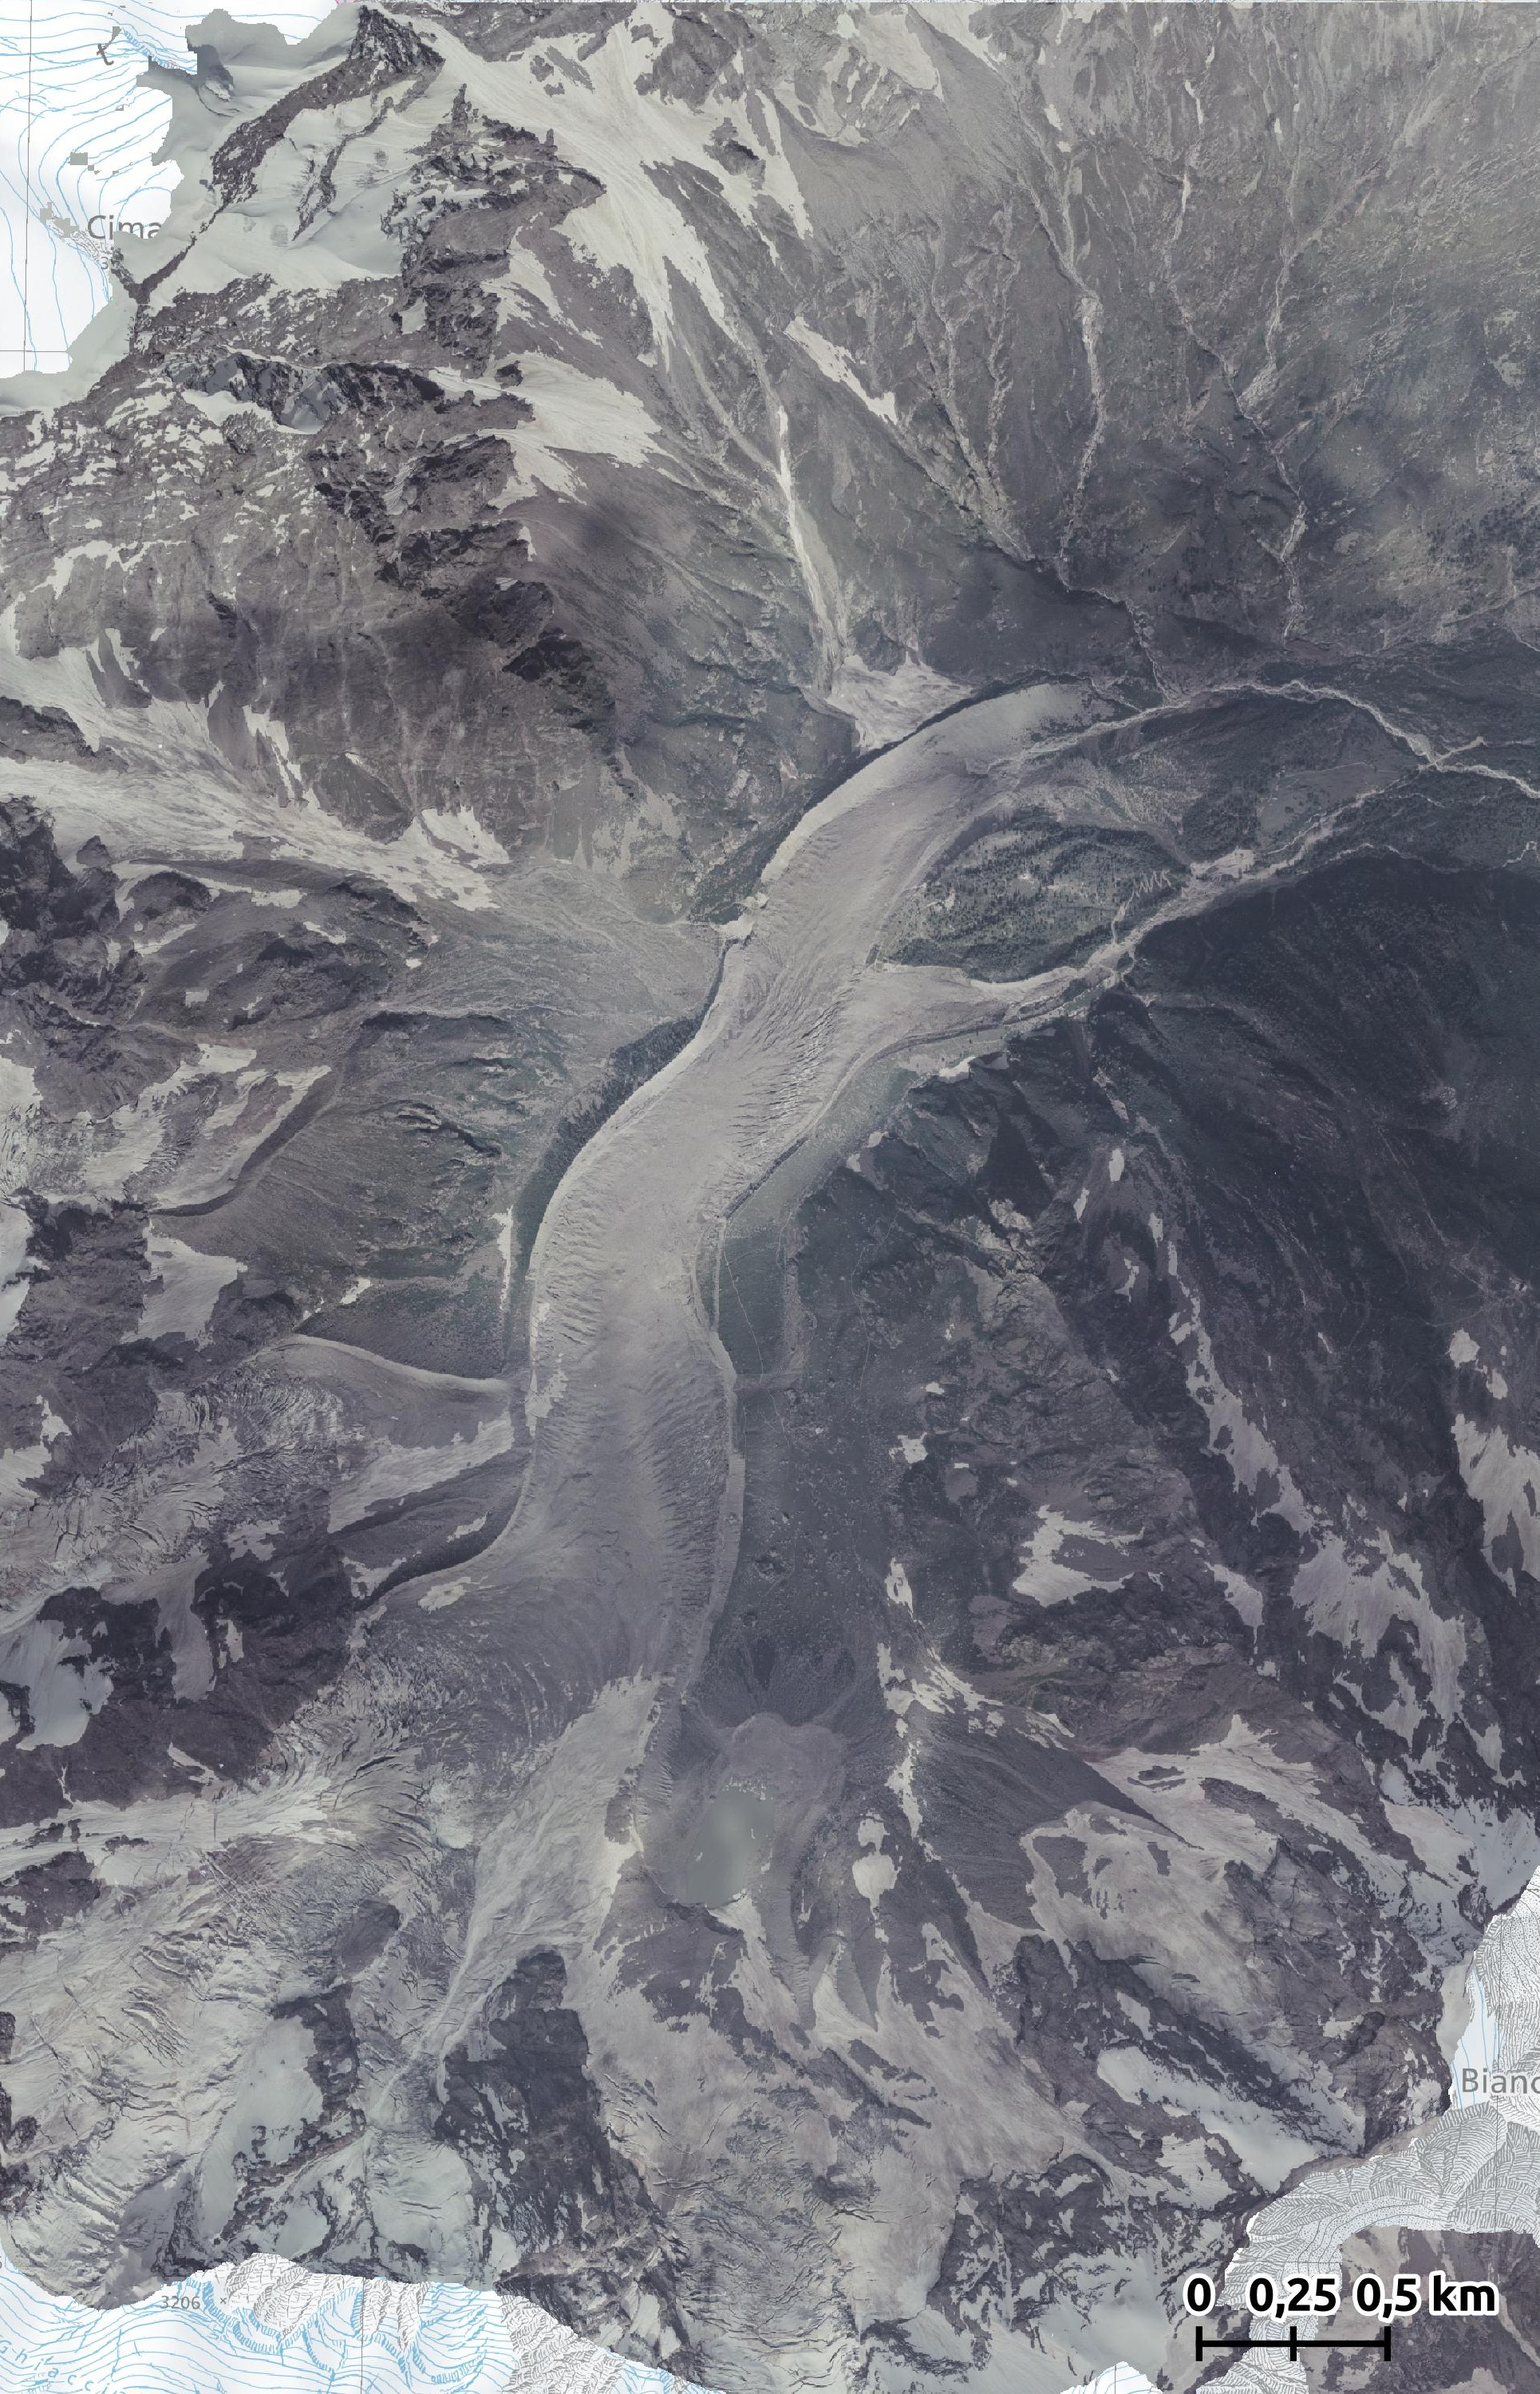
\includegraphics[width=\textwidth]{figures/appendix/orto_1977.jpg}
    \caption{Historical-aerial orthophoto from 1977. Scale 1:25000}
\end{figure}

\begin{figure}[p]
    \centering
    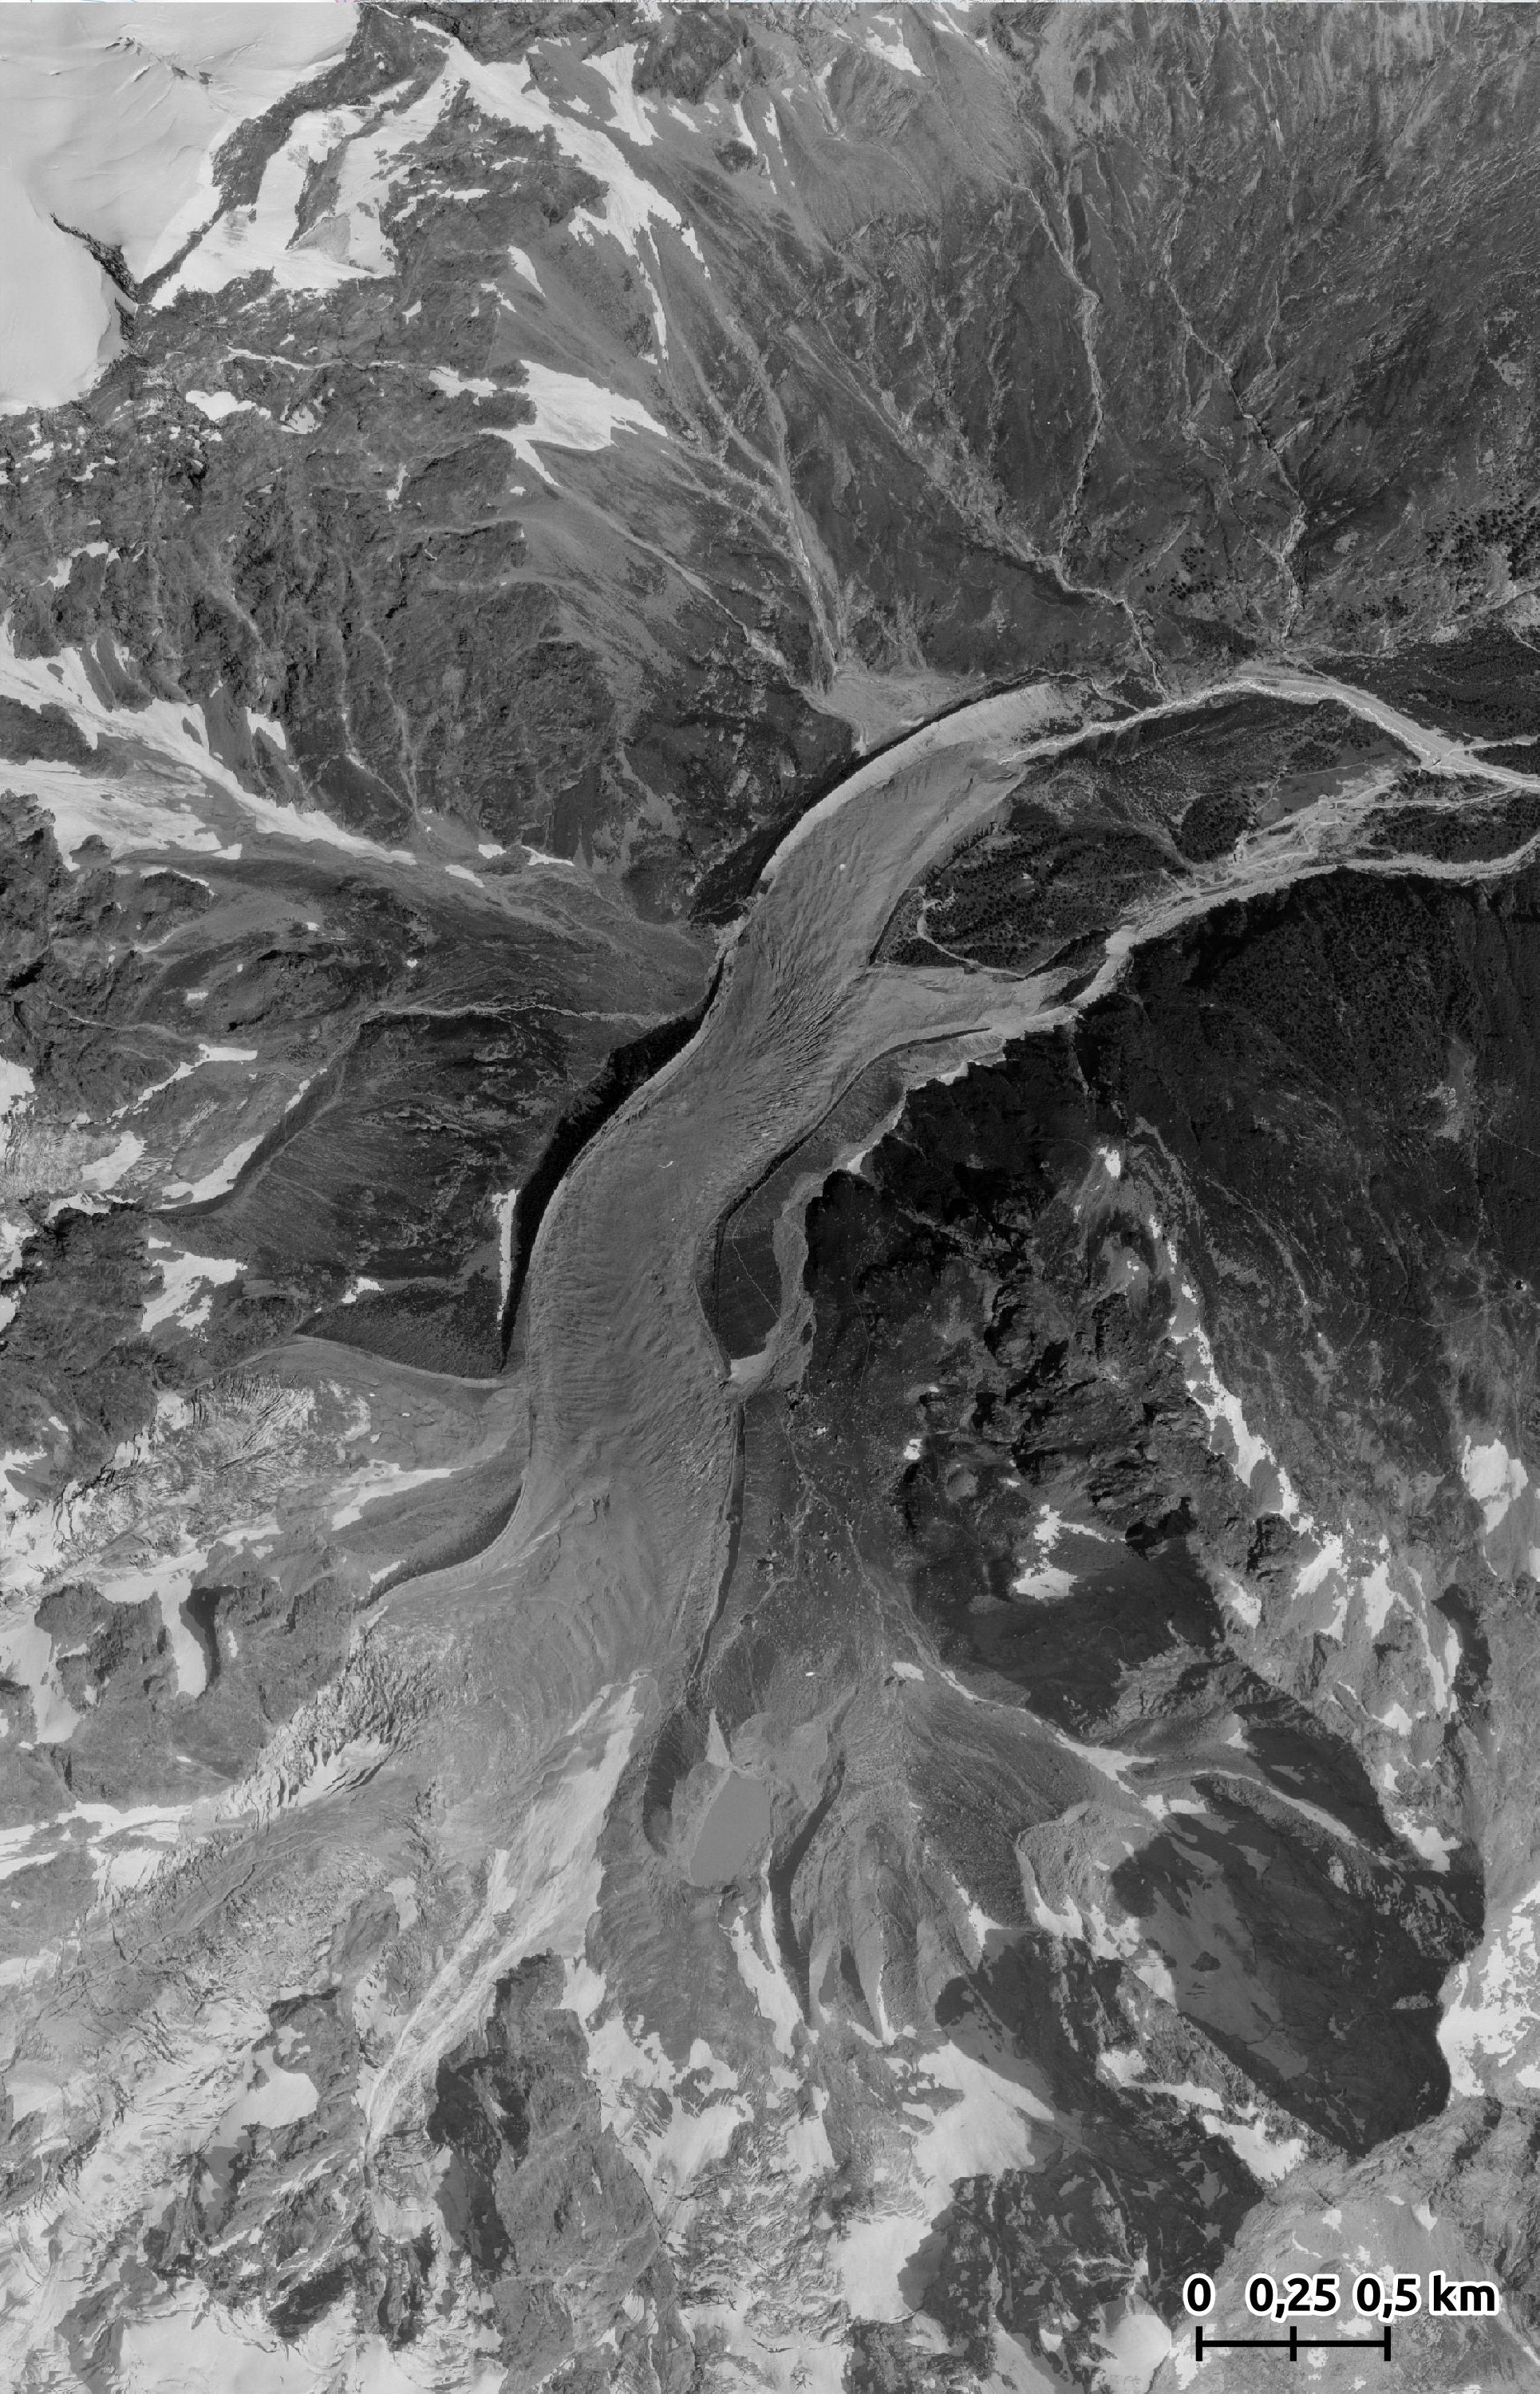
\includegraphics[width=\textwidth]{figures/appendix/orto_1991.jpg}
    \caption{Historical-aerial orthophoto from 1991. Scale 1:25000}
\end{figure}

\begin{figure}[p]
    \centering
    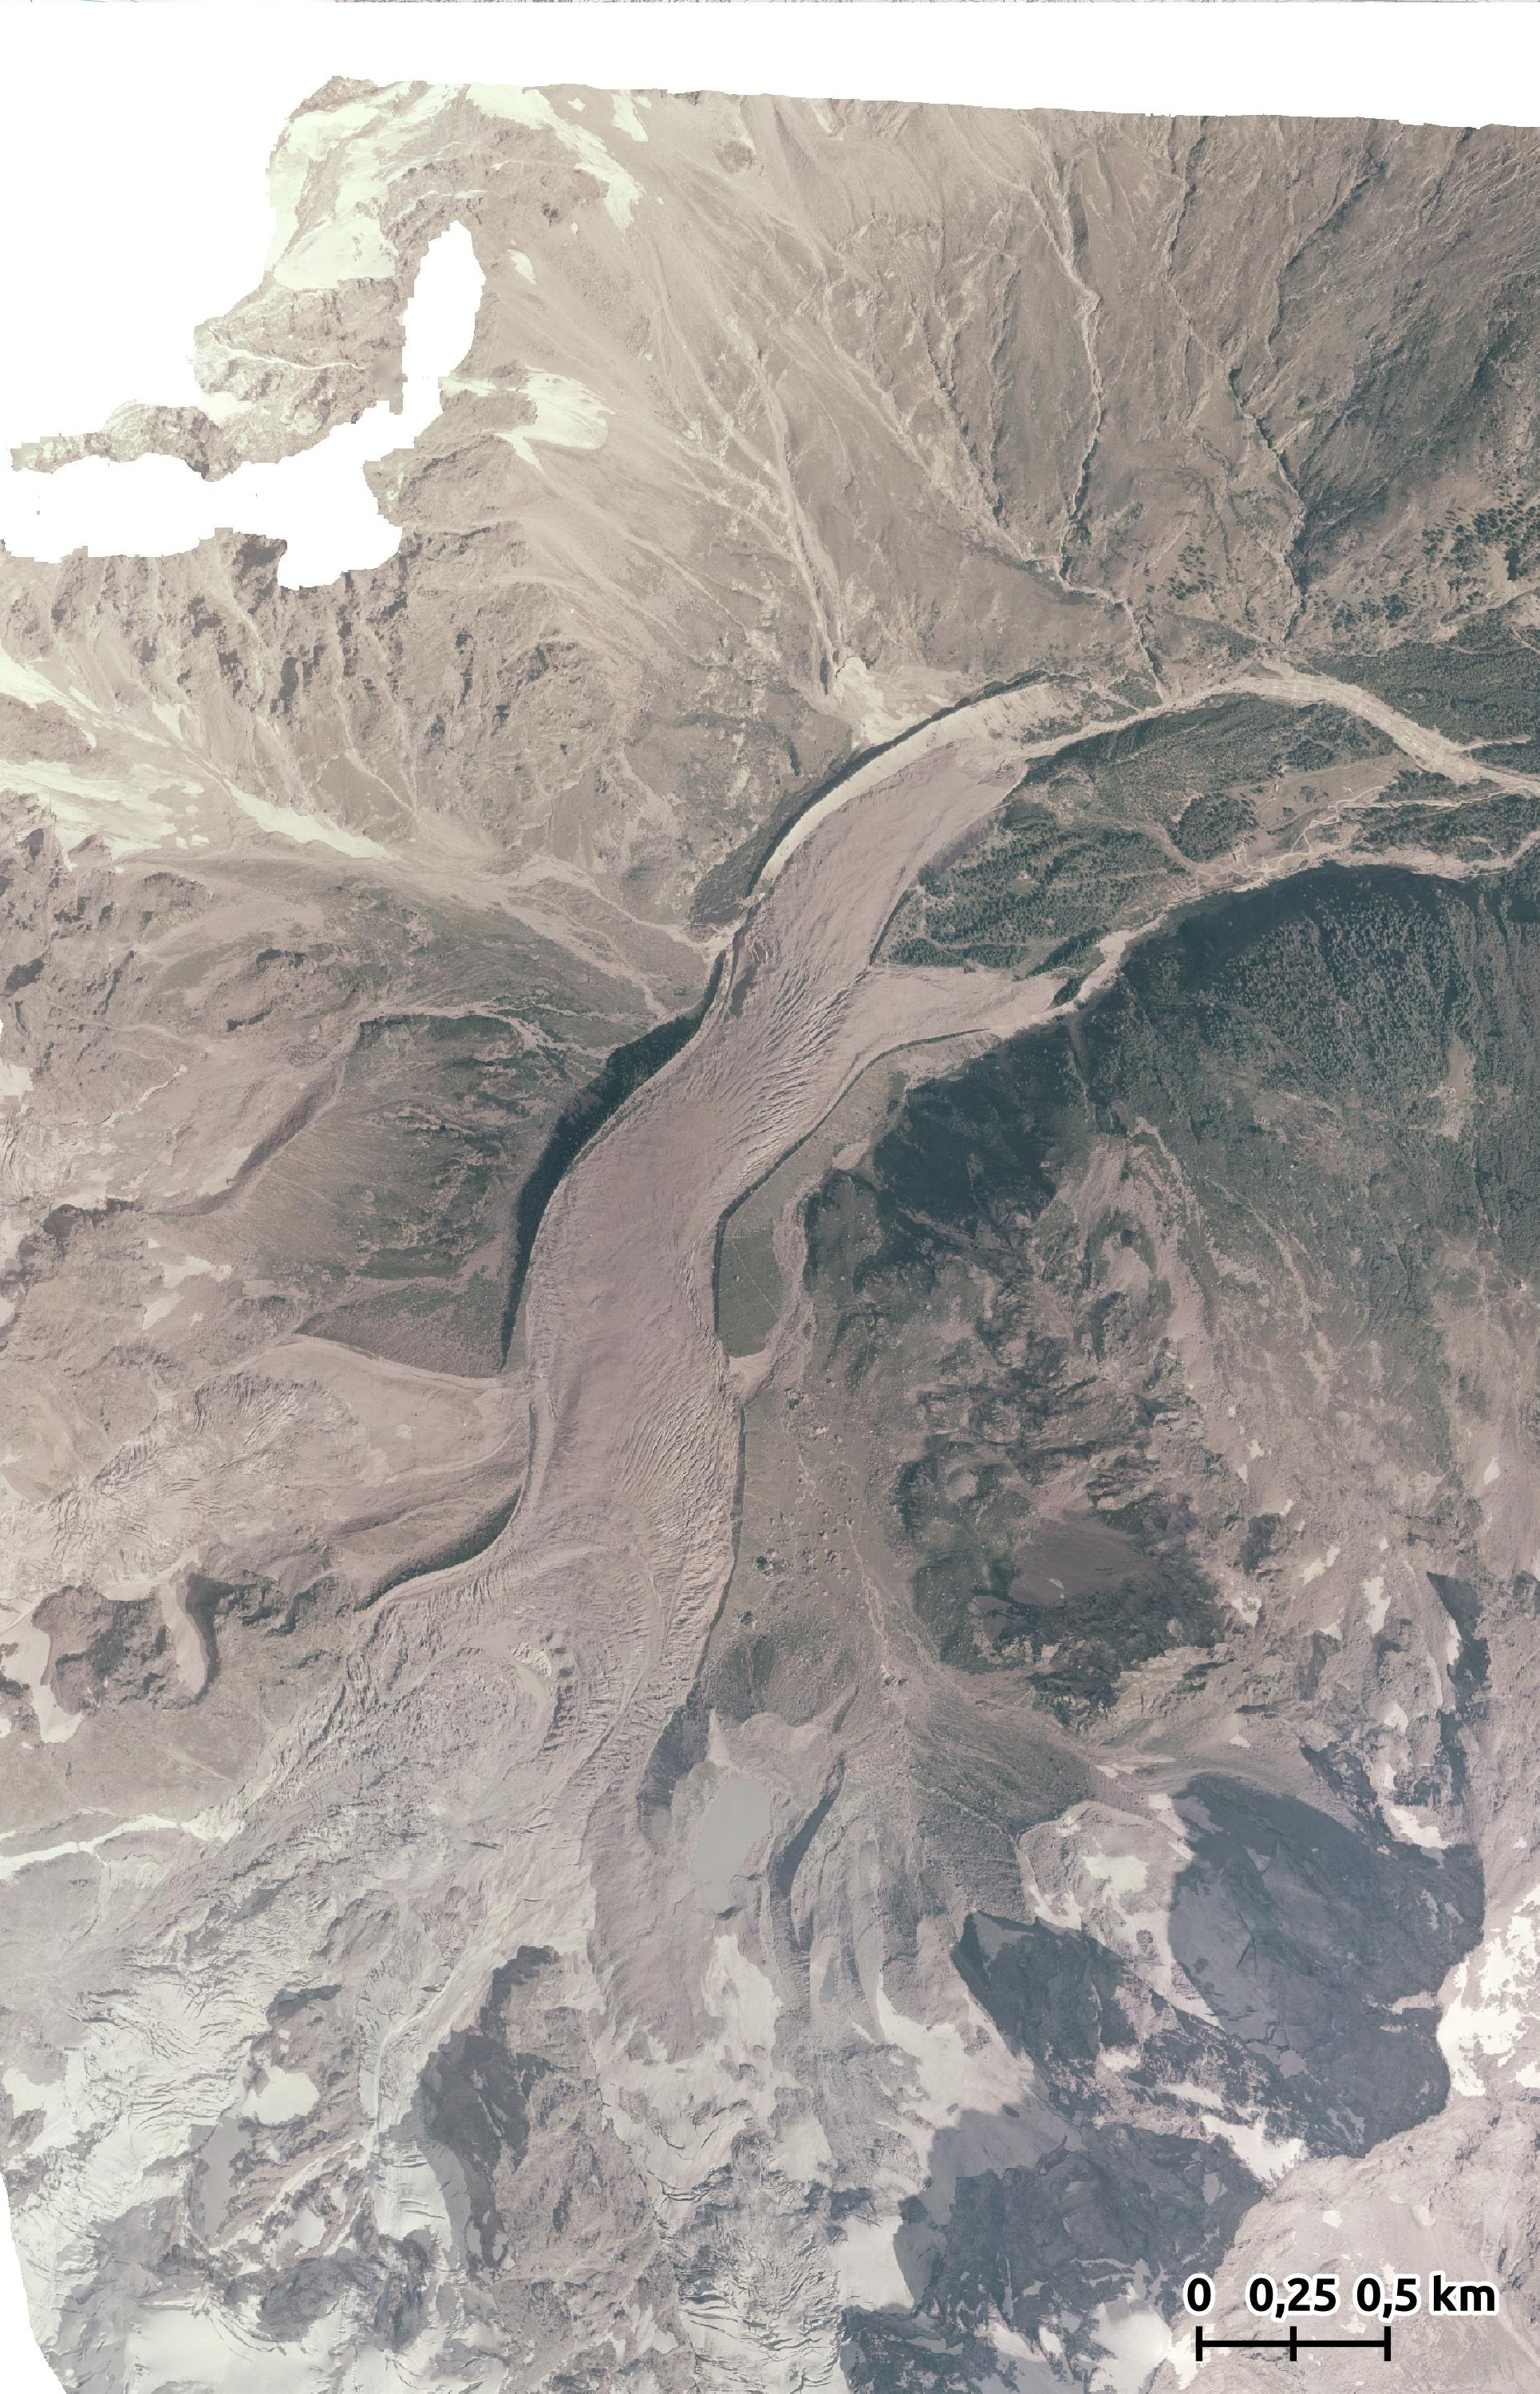
\includegraphics[width=\textwidth]{figures/appendix/orto_2001.jpg}
    \caption{Historical-aerial orthophoto from 2001. Scale 1:25000}
\end{figure}

\begin{figure}[p]
    \centering
    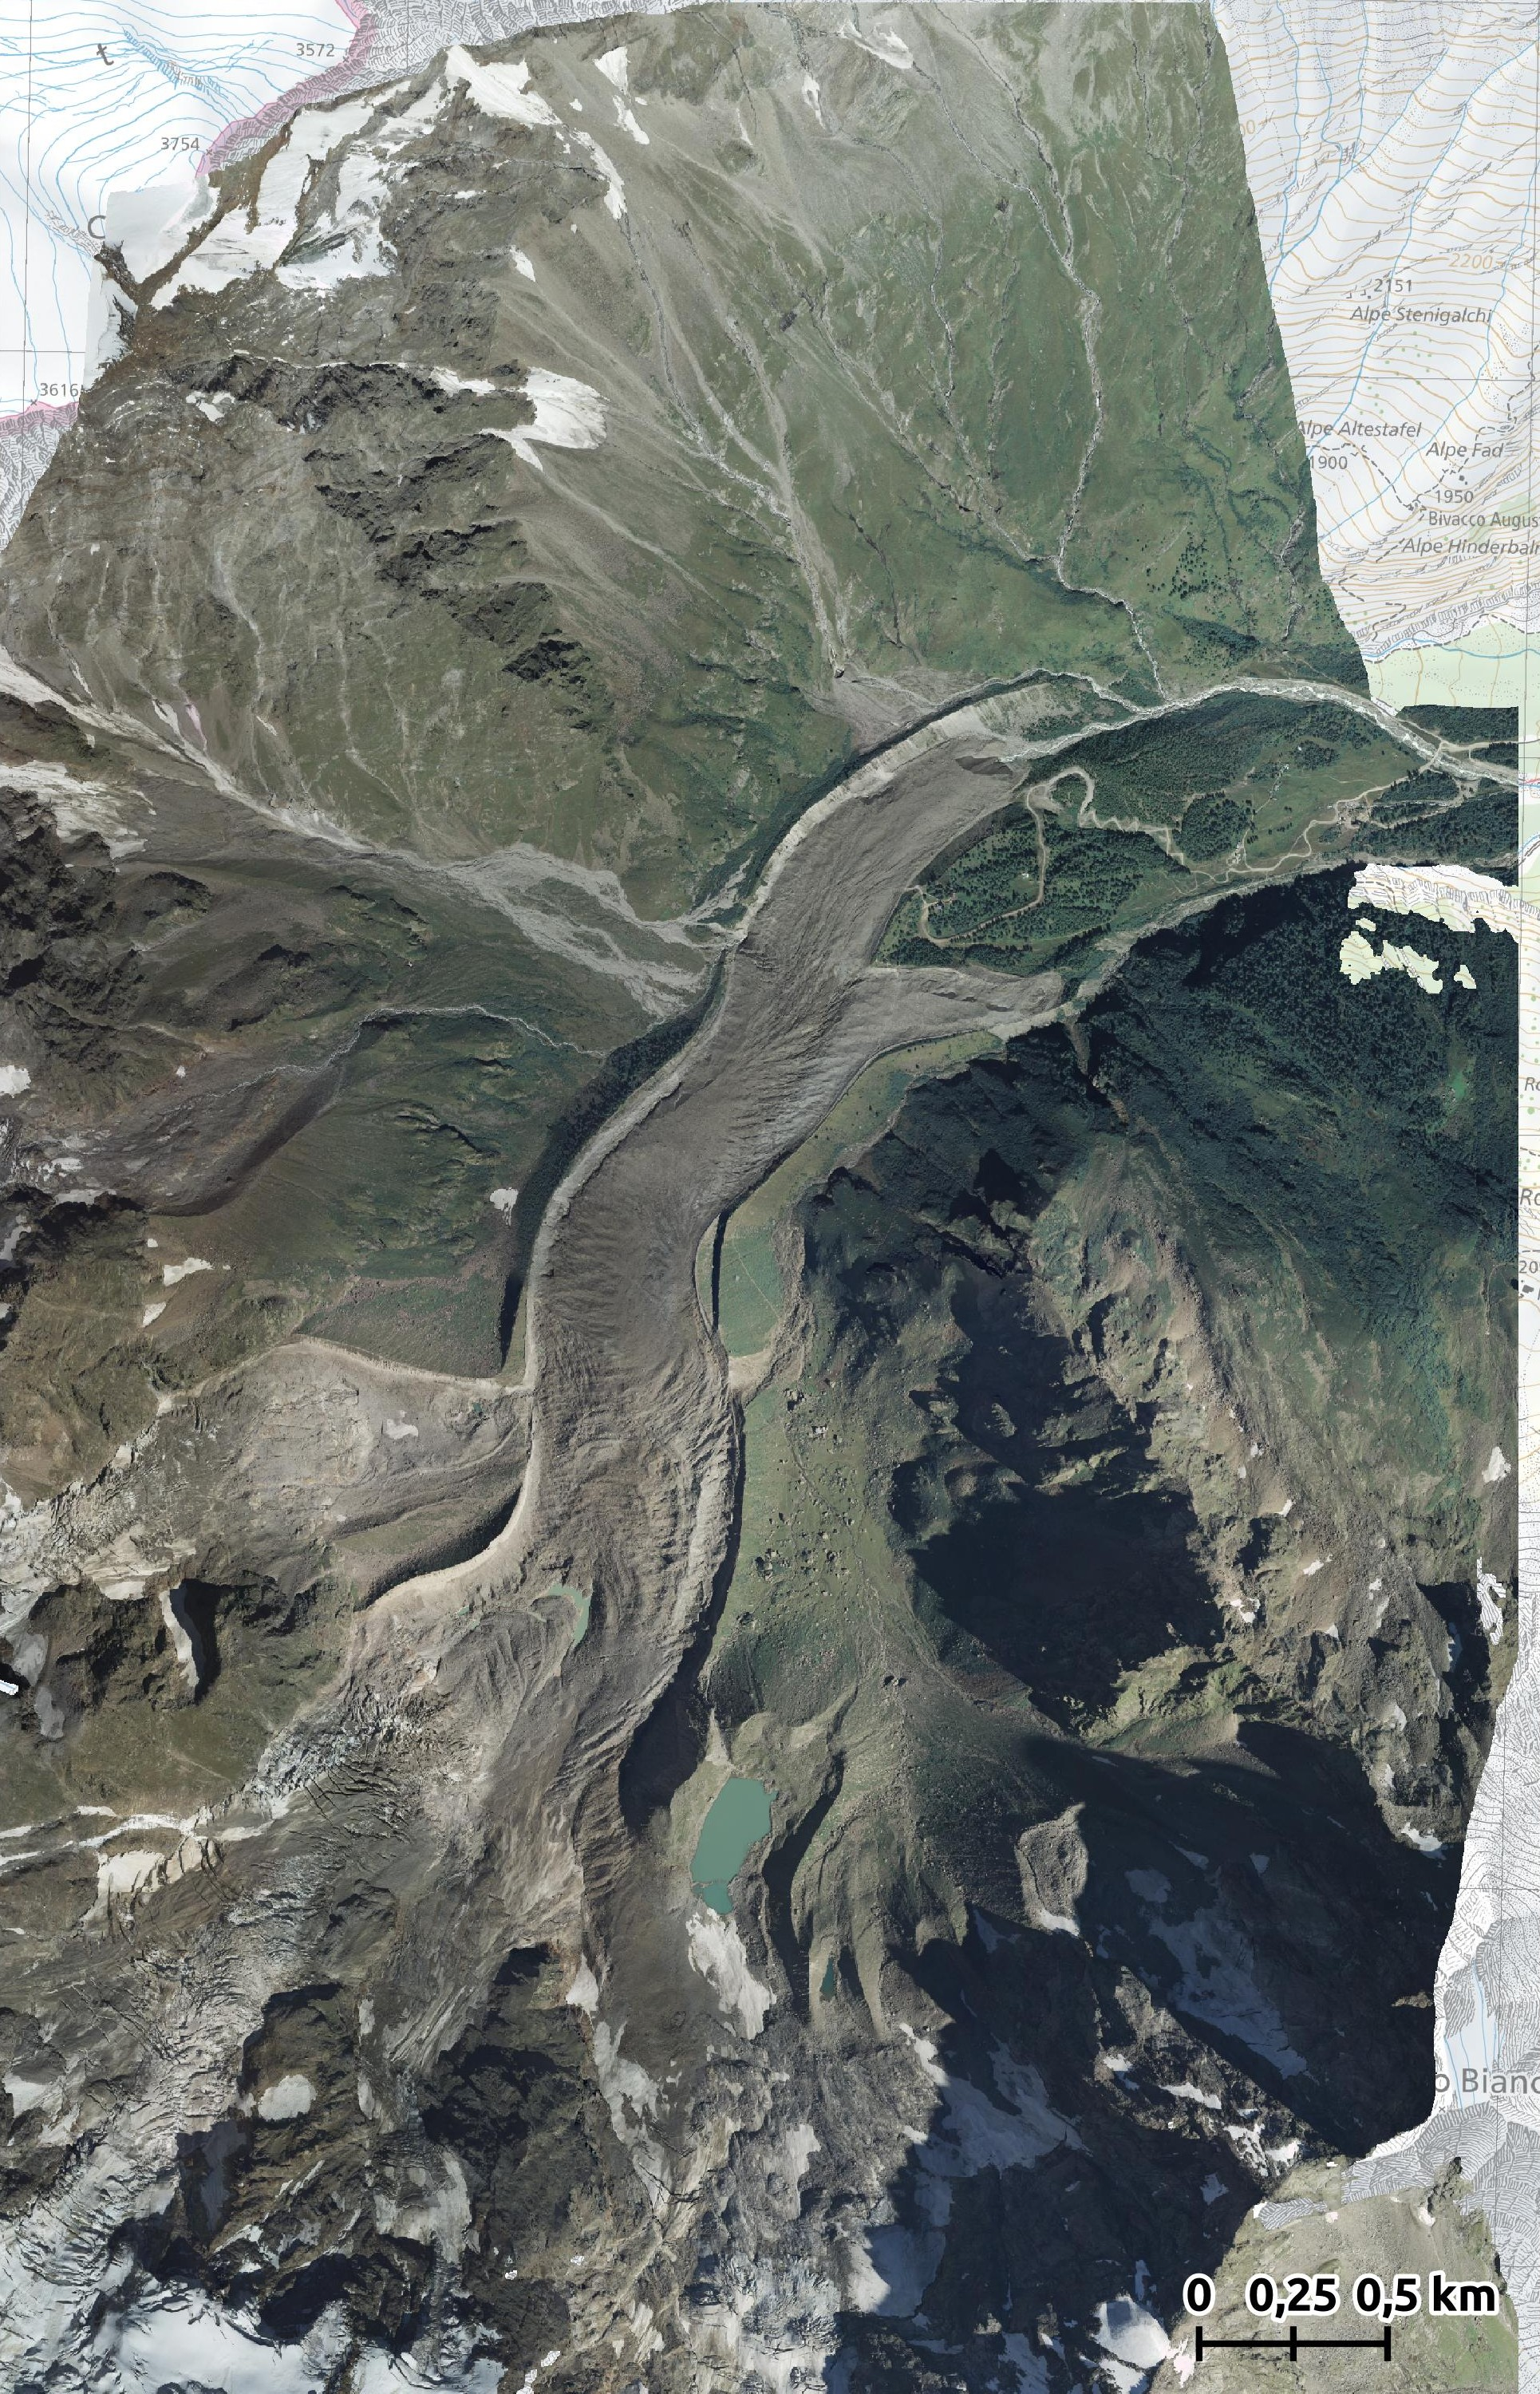
\includegraphics[width=\textwidth]{figures/appendix/orto_2009.jpg}
    \caption{Aerial orthophoto from 2009. Scale 1:25000}
\end{figure}

\begin{figure}[p]
    \centering
    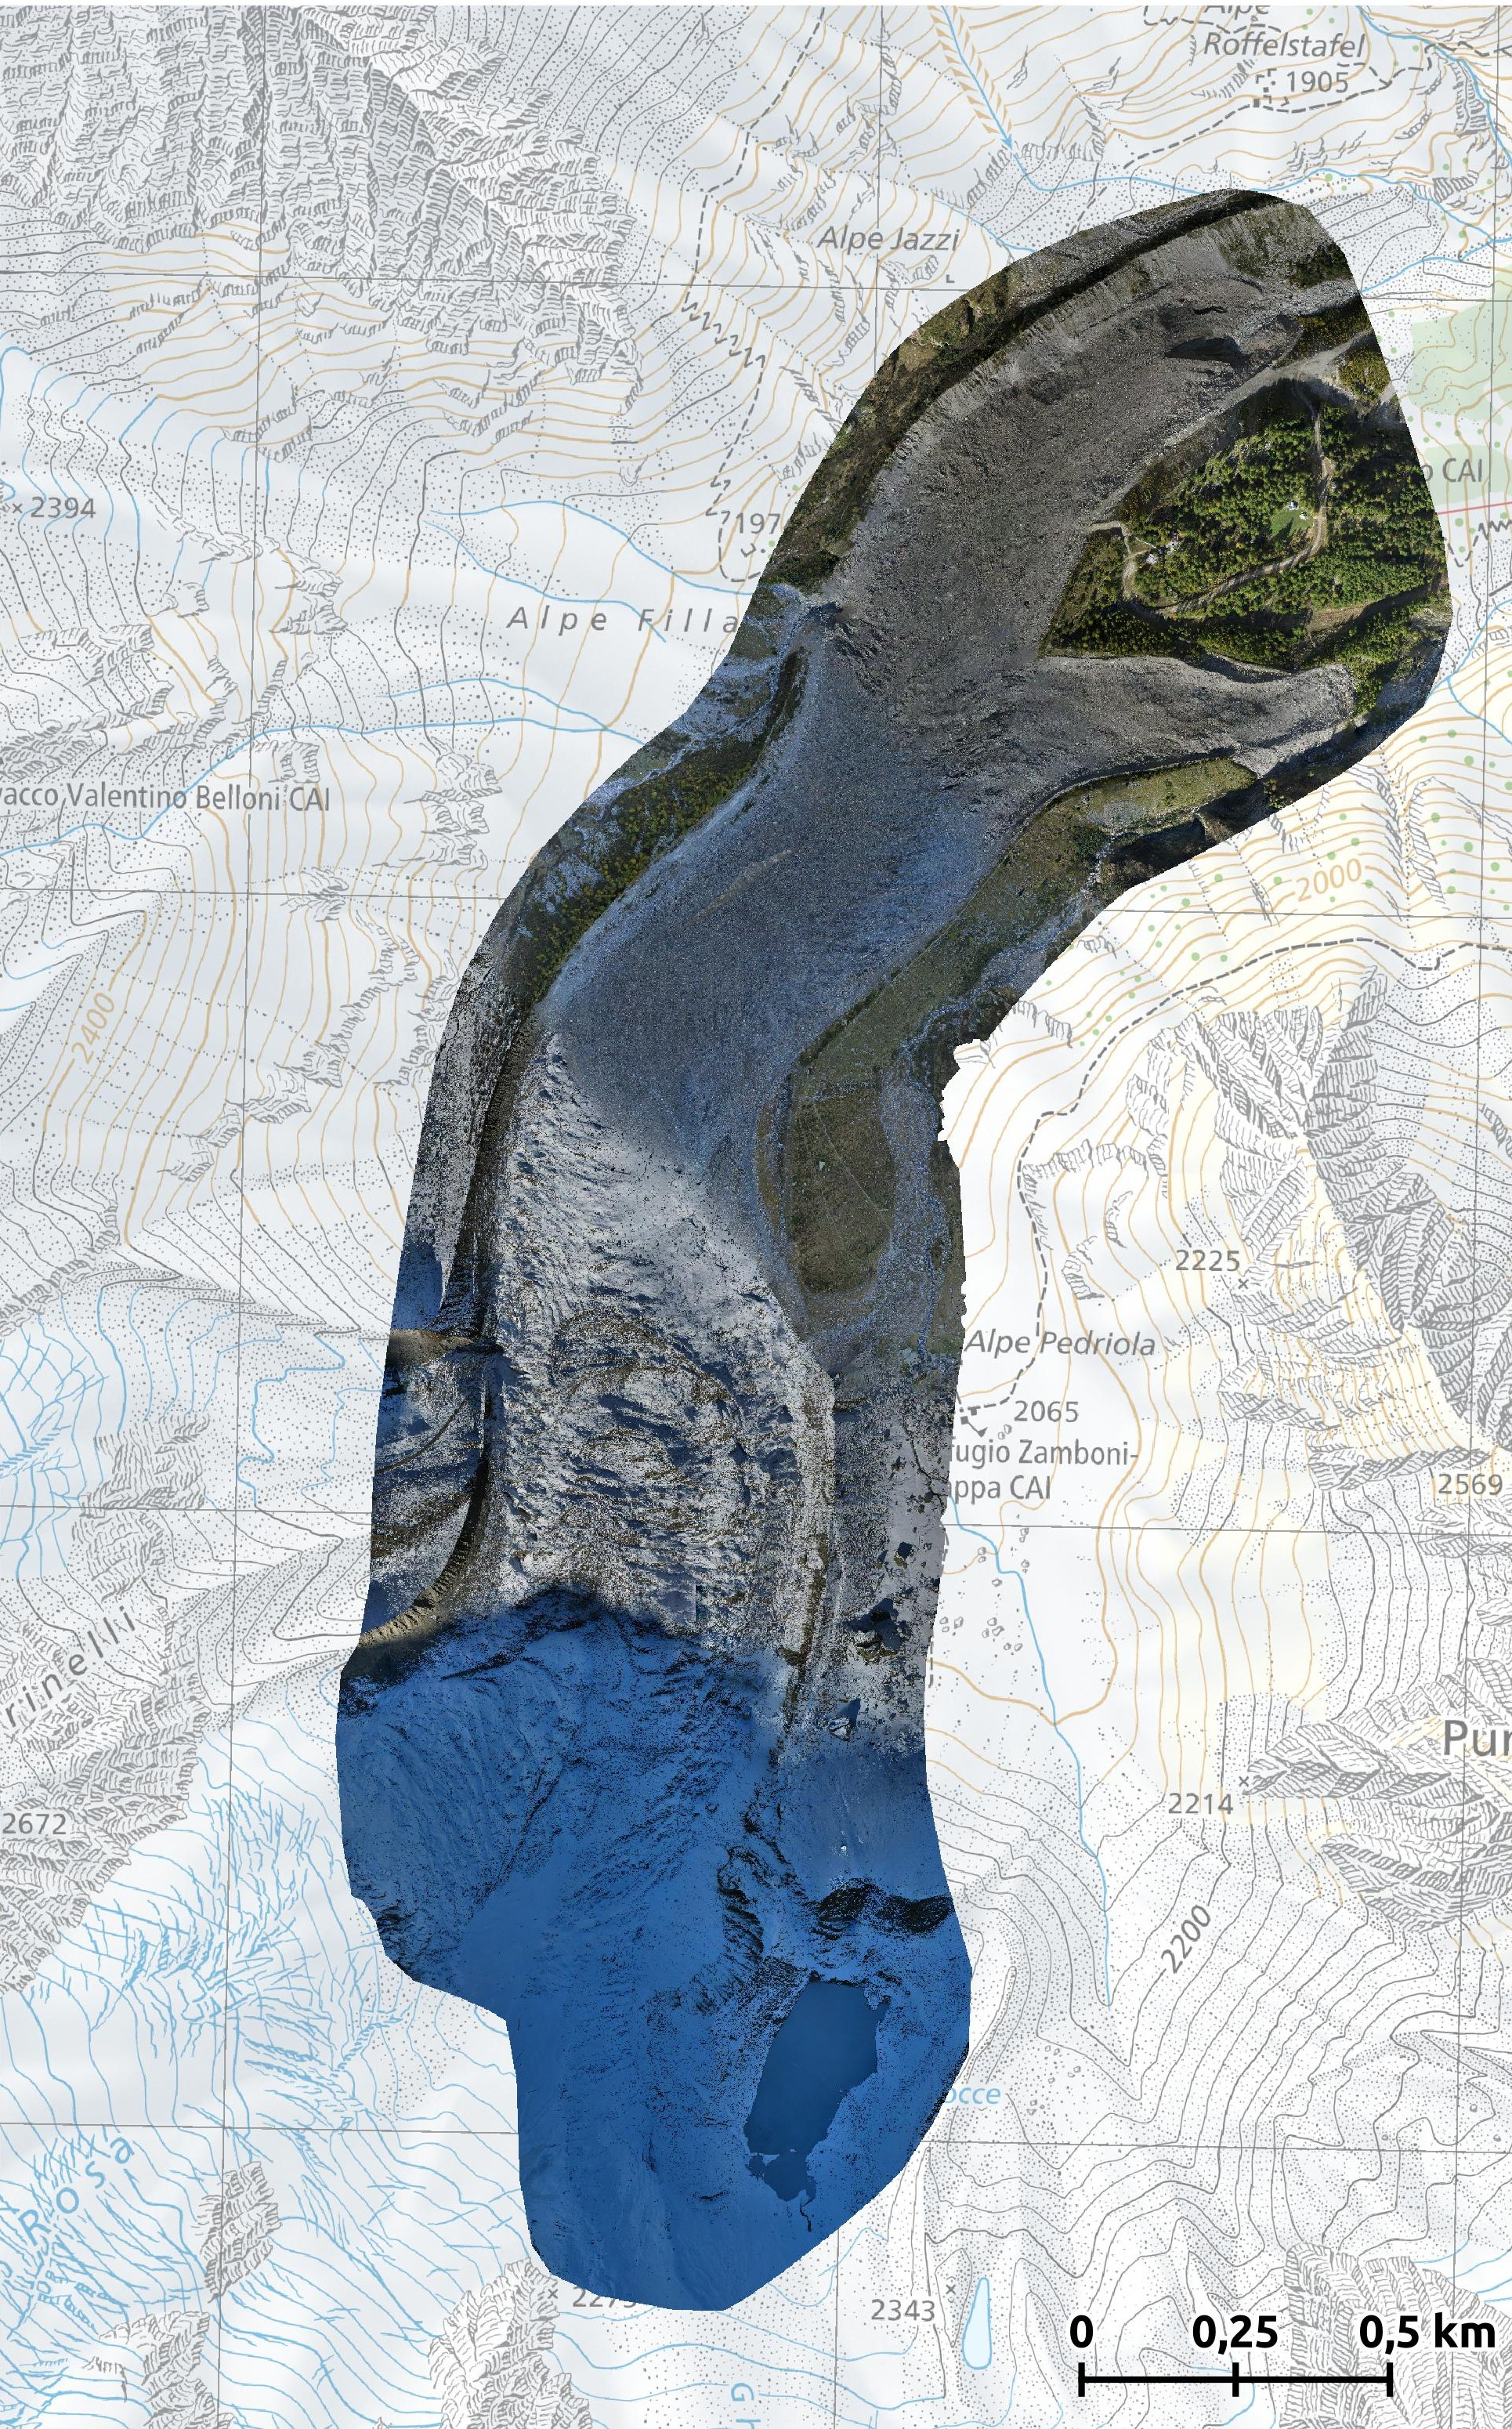
\includegraphics[width=\textwidth]{figures/appendix/orto_2015.jpg}
    \caption{UAV orthophoto from 2015. Scale 1:15000}
\end{figure}

\begin{figure}[p]
    \centering
    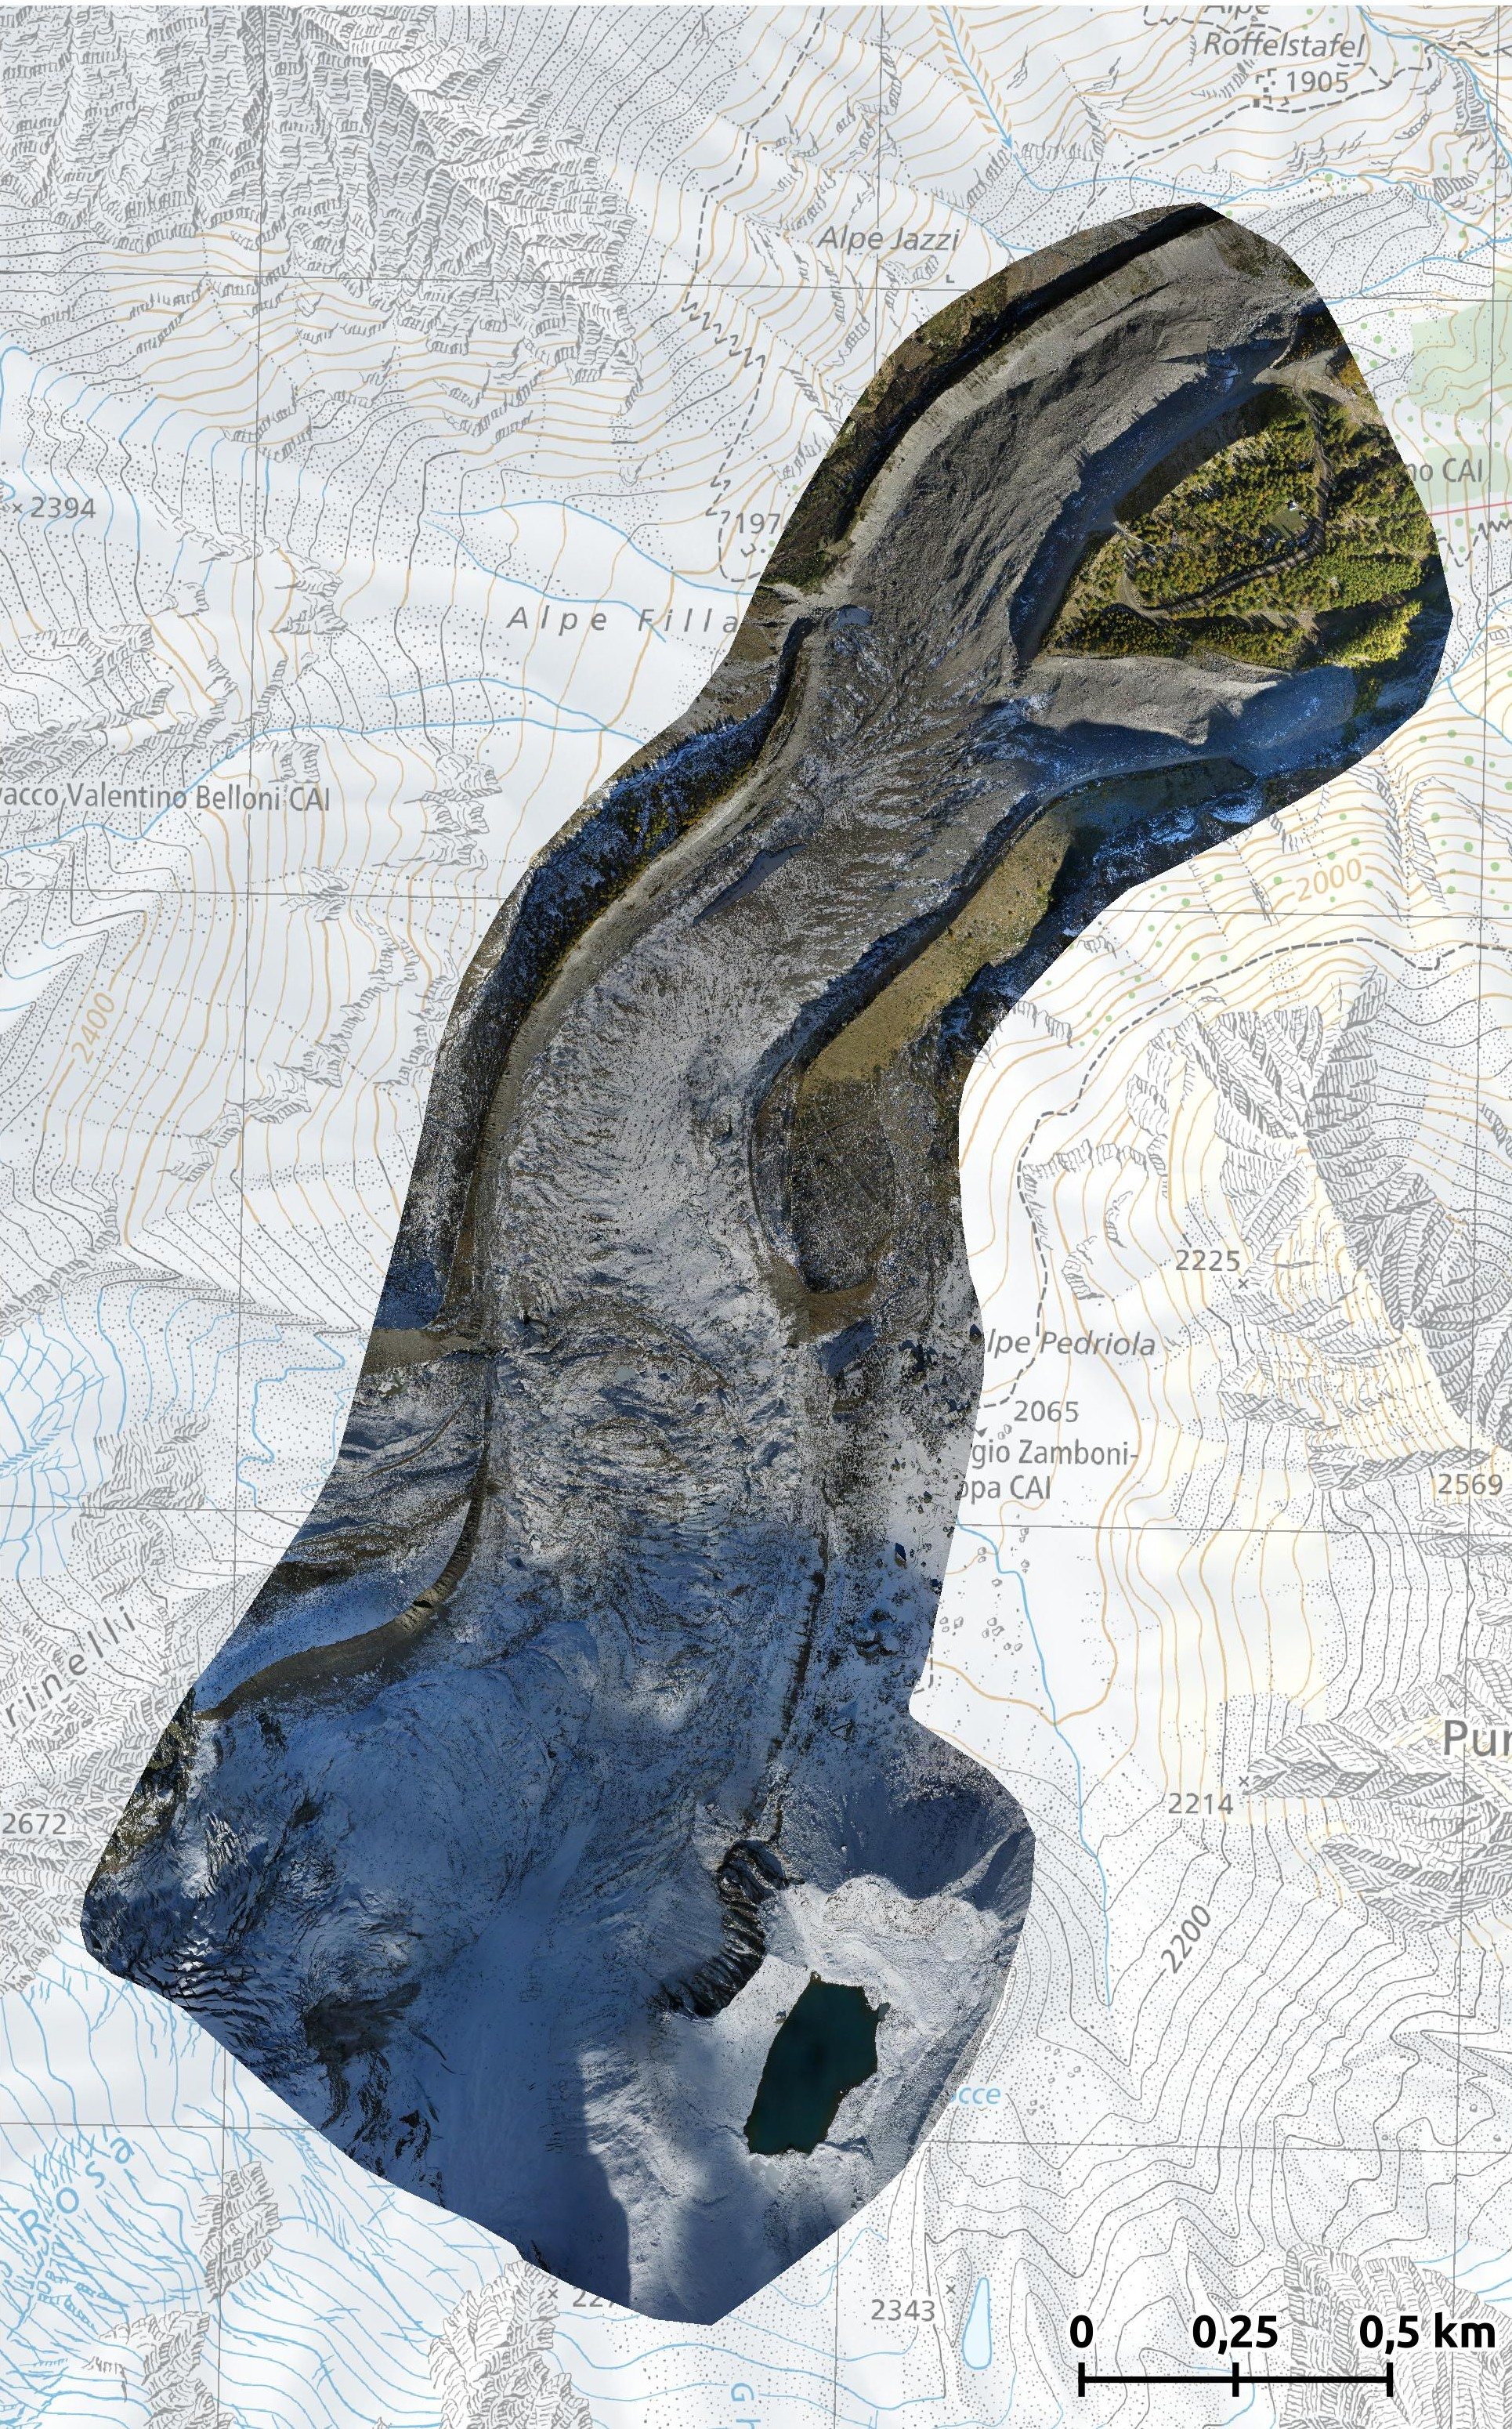
\includegraphics[width=\textwidth]{figures/appendix/orto_2016.jpg}
    \caption{UAV orthophoto from 2016. Scale 1:15000}
\end{figure}

\begin{figure}[p]
    \centering
    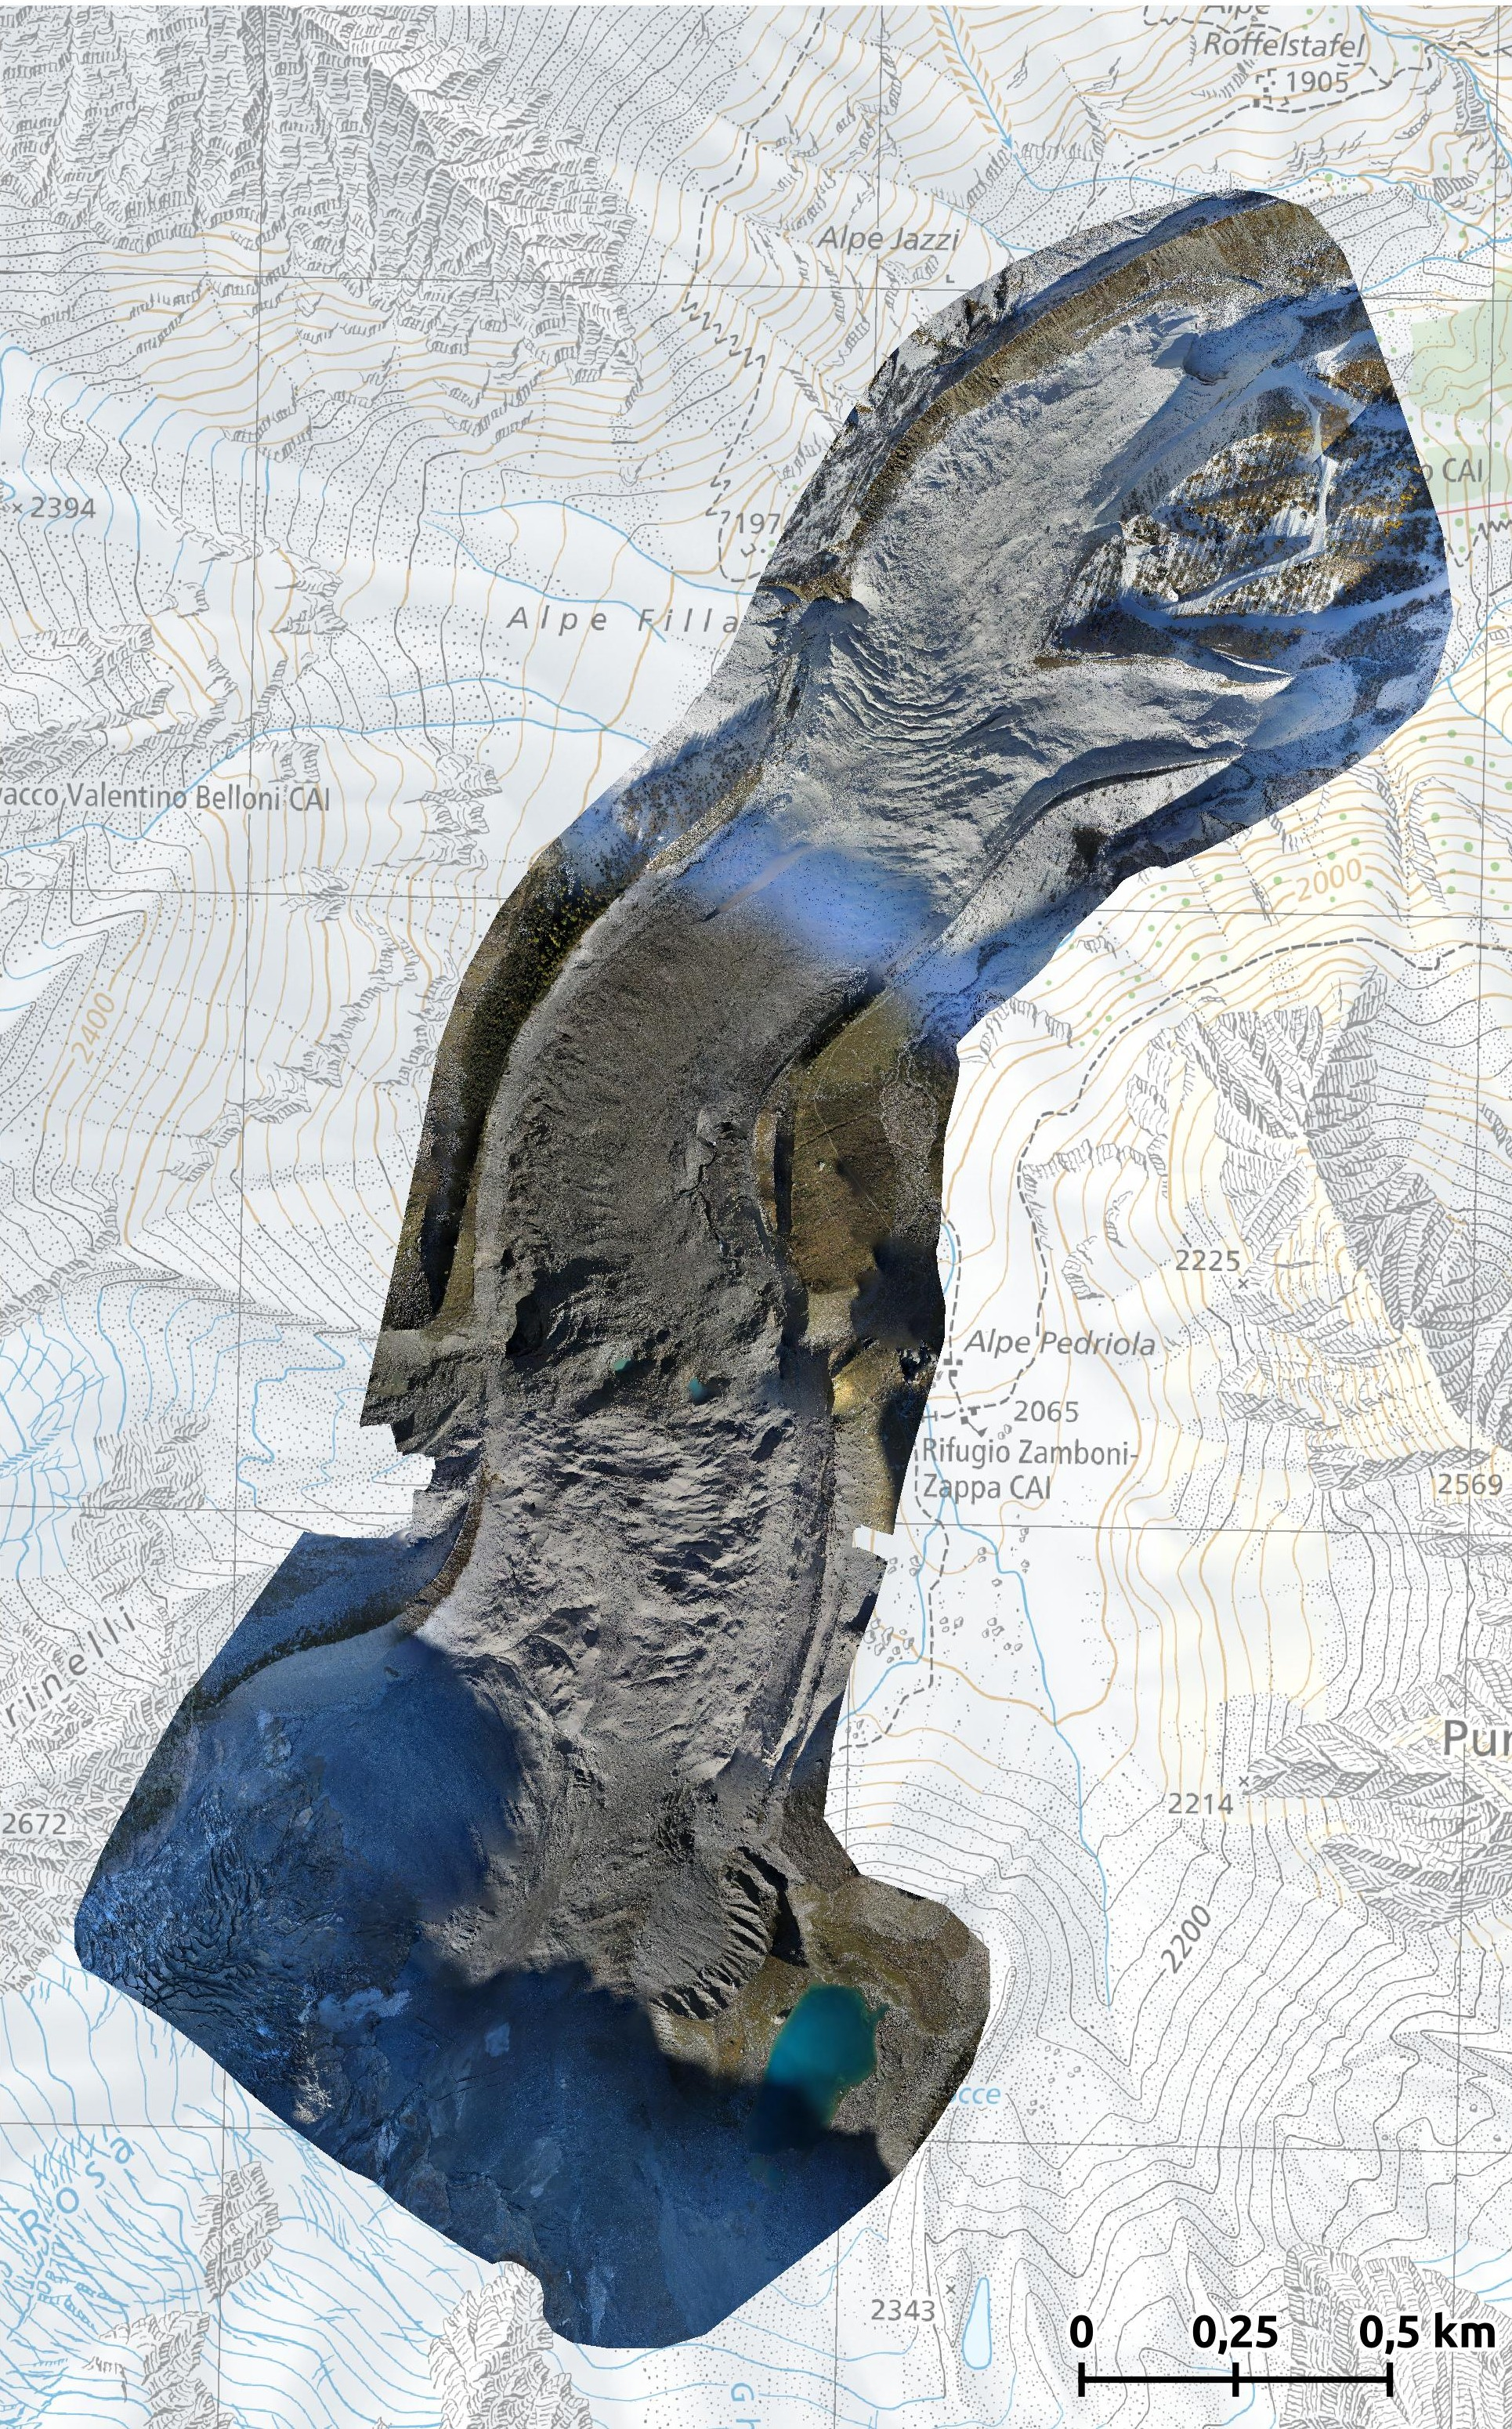
\includegraphics[width=\textwidth]{figures/appendix/orto_2017.jpg}
    \caption{UAV orthophoto from 2017. Scale 1:15000}
\end{figure}

\begin{figure}[p]
    \centering
    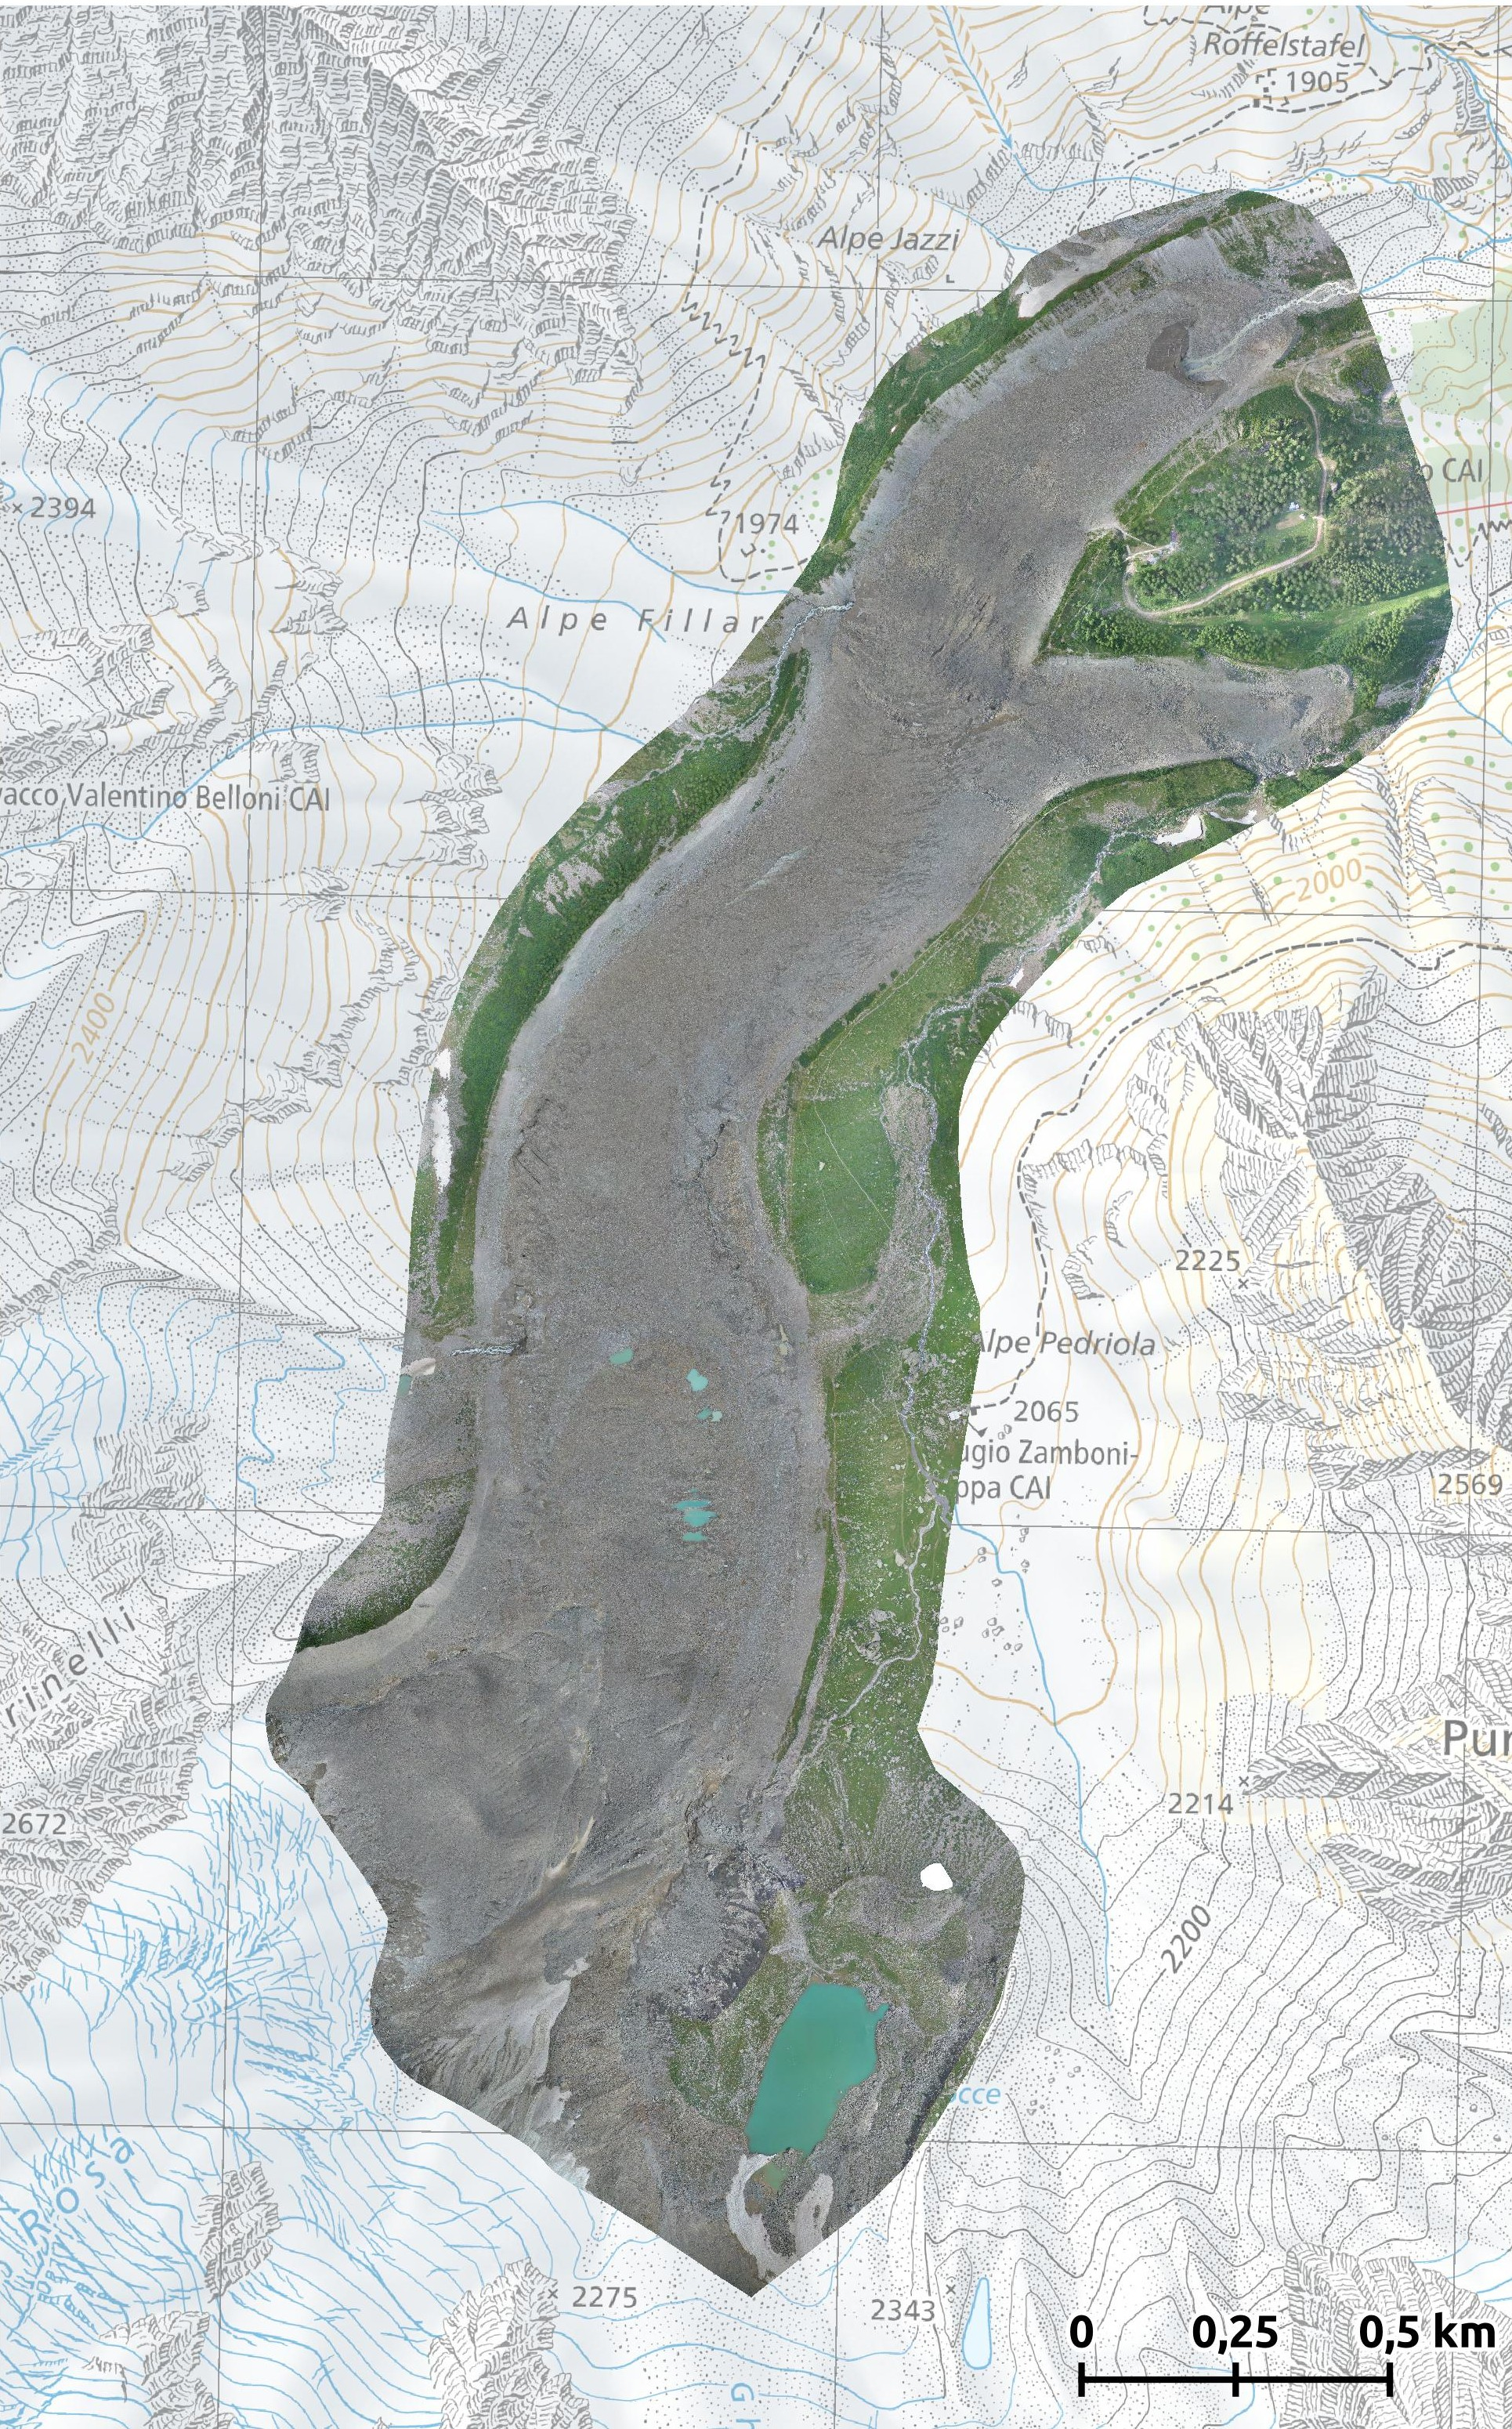
\includegraphics[width=\textwidth]{figures/appendix/orto_2018.jpg}
    \caption{UAV orthophoto from 2018. Scale 1:15000}
\end{figure}

\begin{figure}[p]
    \centering
    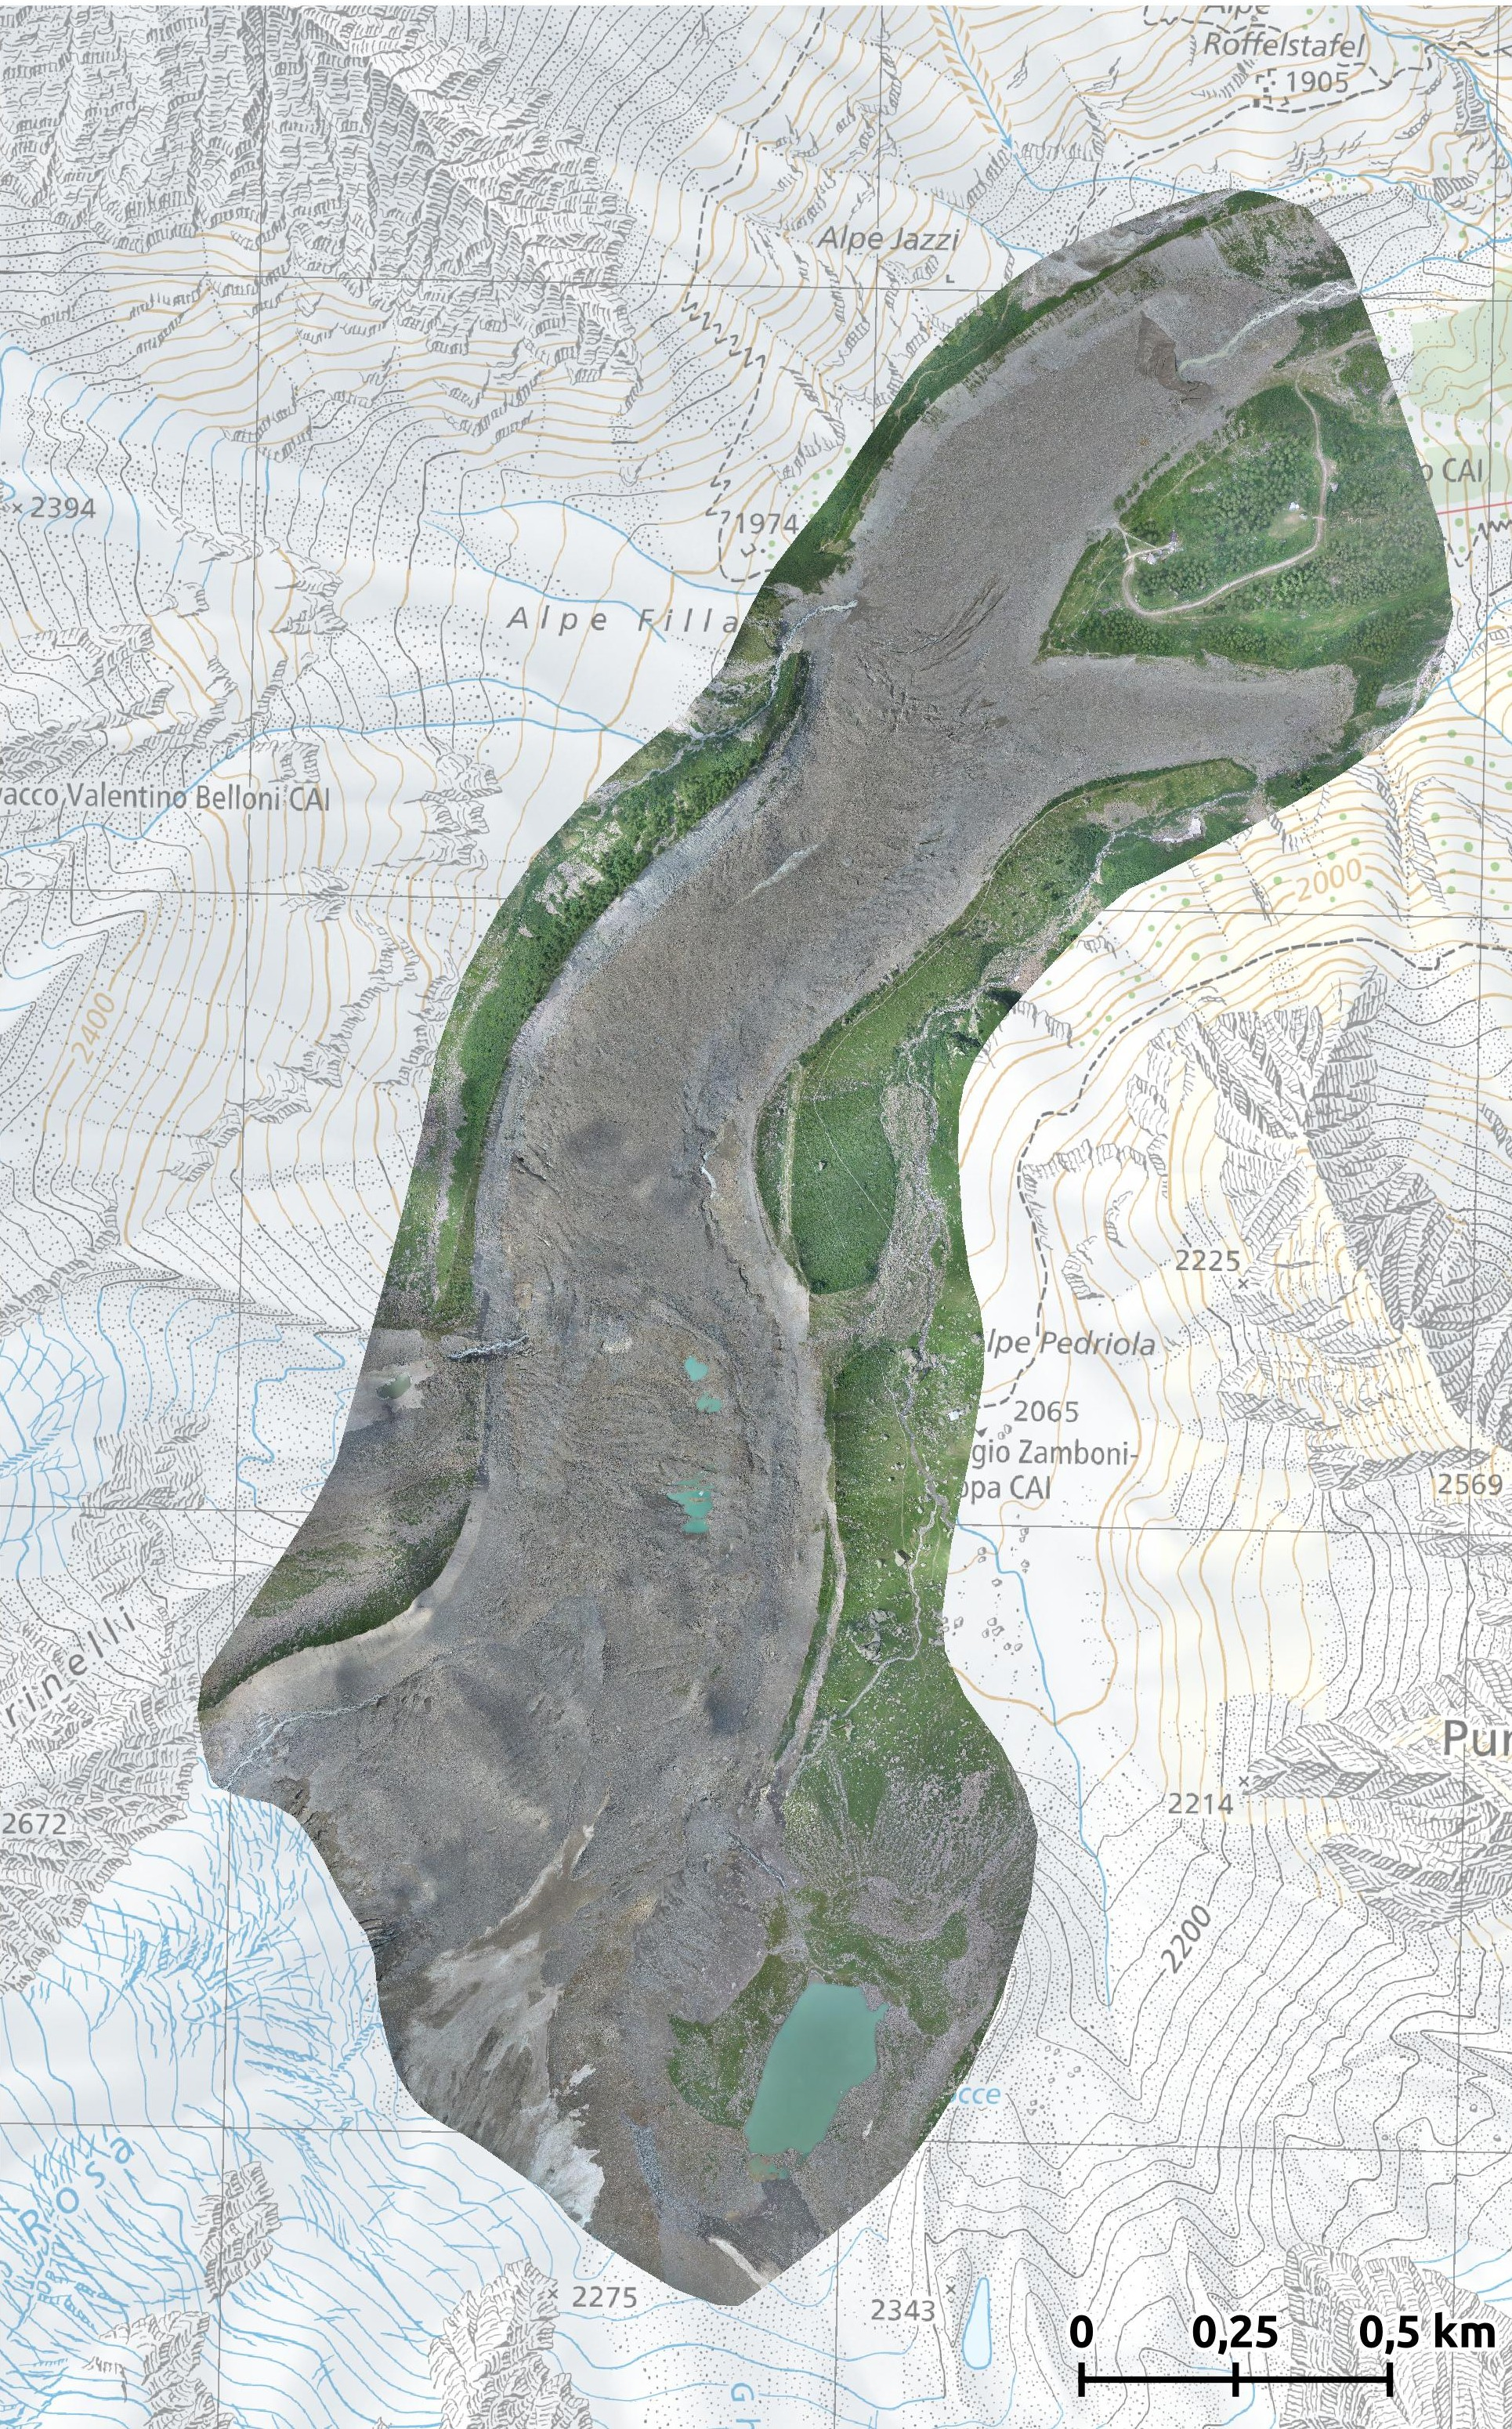
\includegraphics[width=\textwidth]{figures/appendix/orto_2019.jpg}
    \caption{UAV orthophoto from 2019. Scale 1:15000}
\end{figure}

\begin{figure}[p]
    \centering
    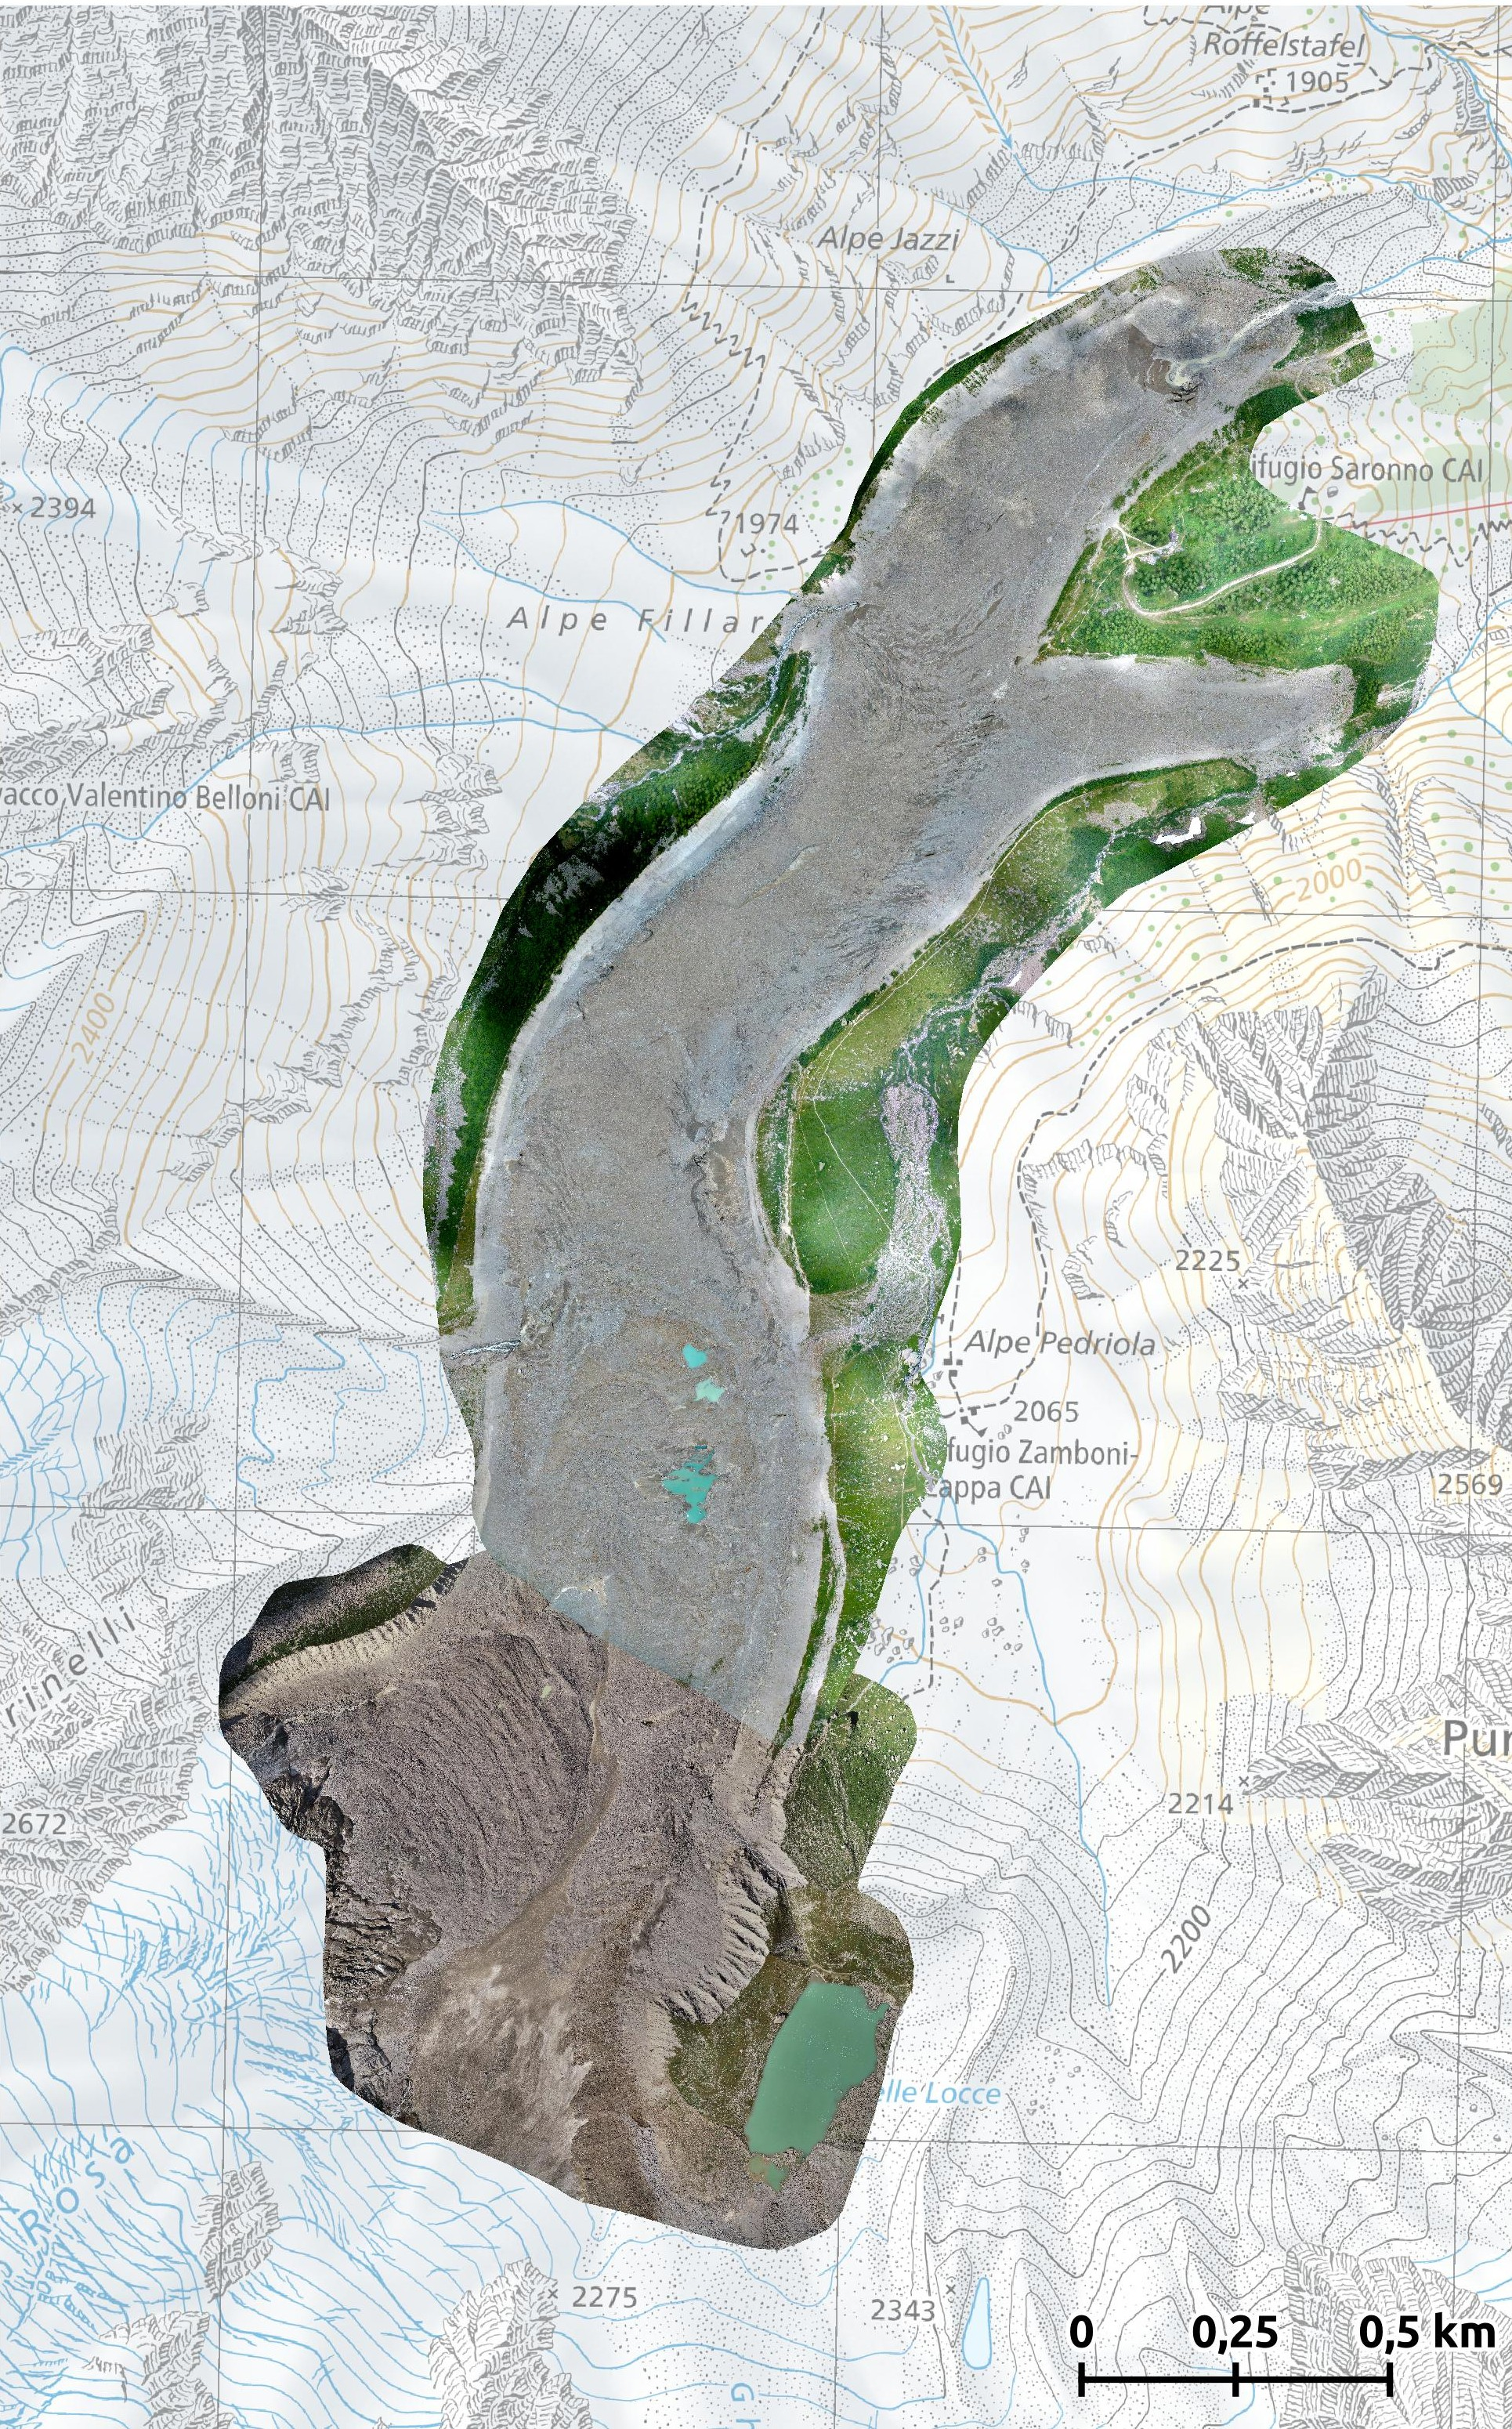
\includegraphics[width=\textwidth]{figures/appendix/orto_2020.jpg}
    \caption{UAV orthophoto from 2020. Scale 1:15000}
\end{figure}

\begin{figure}[p]
    \centering
    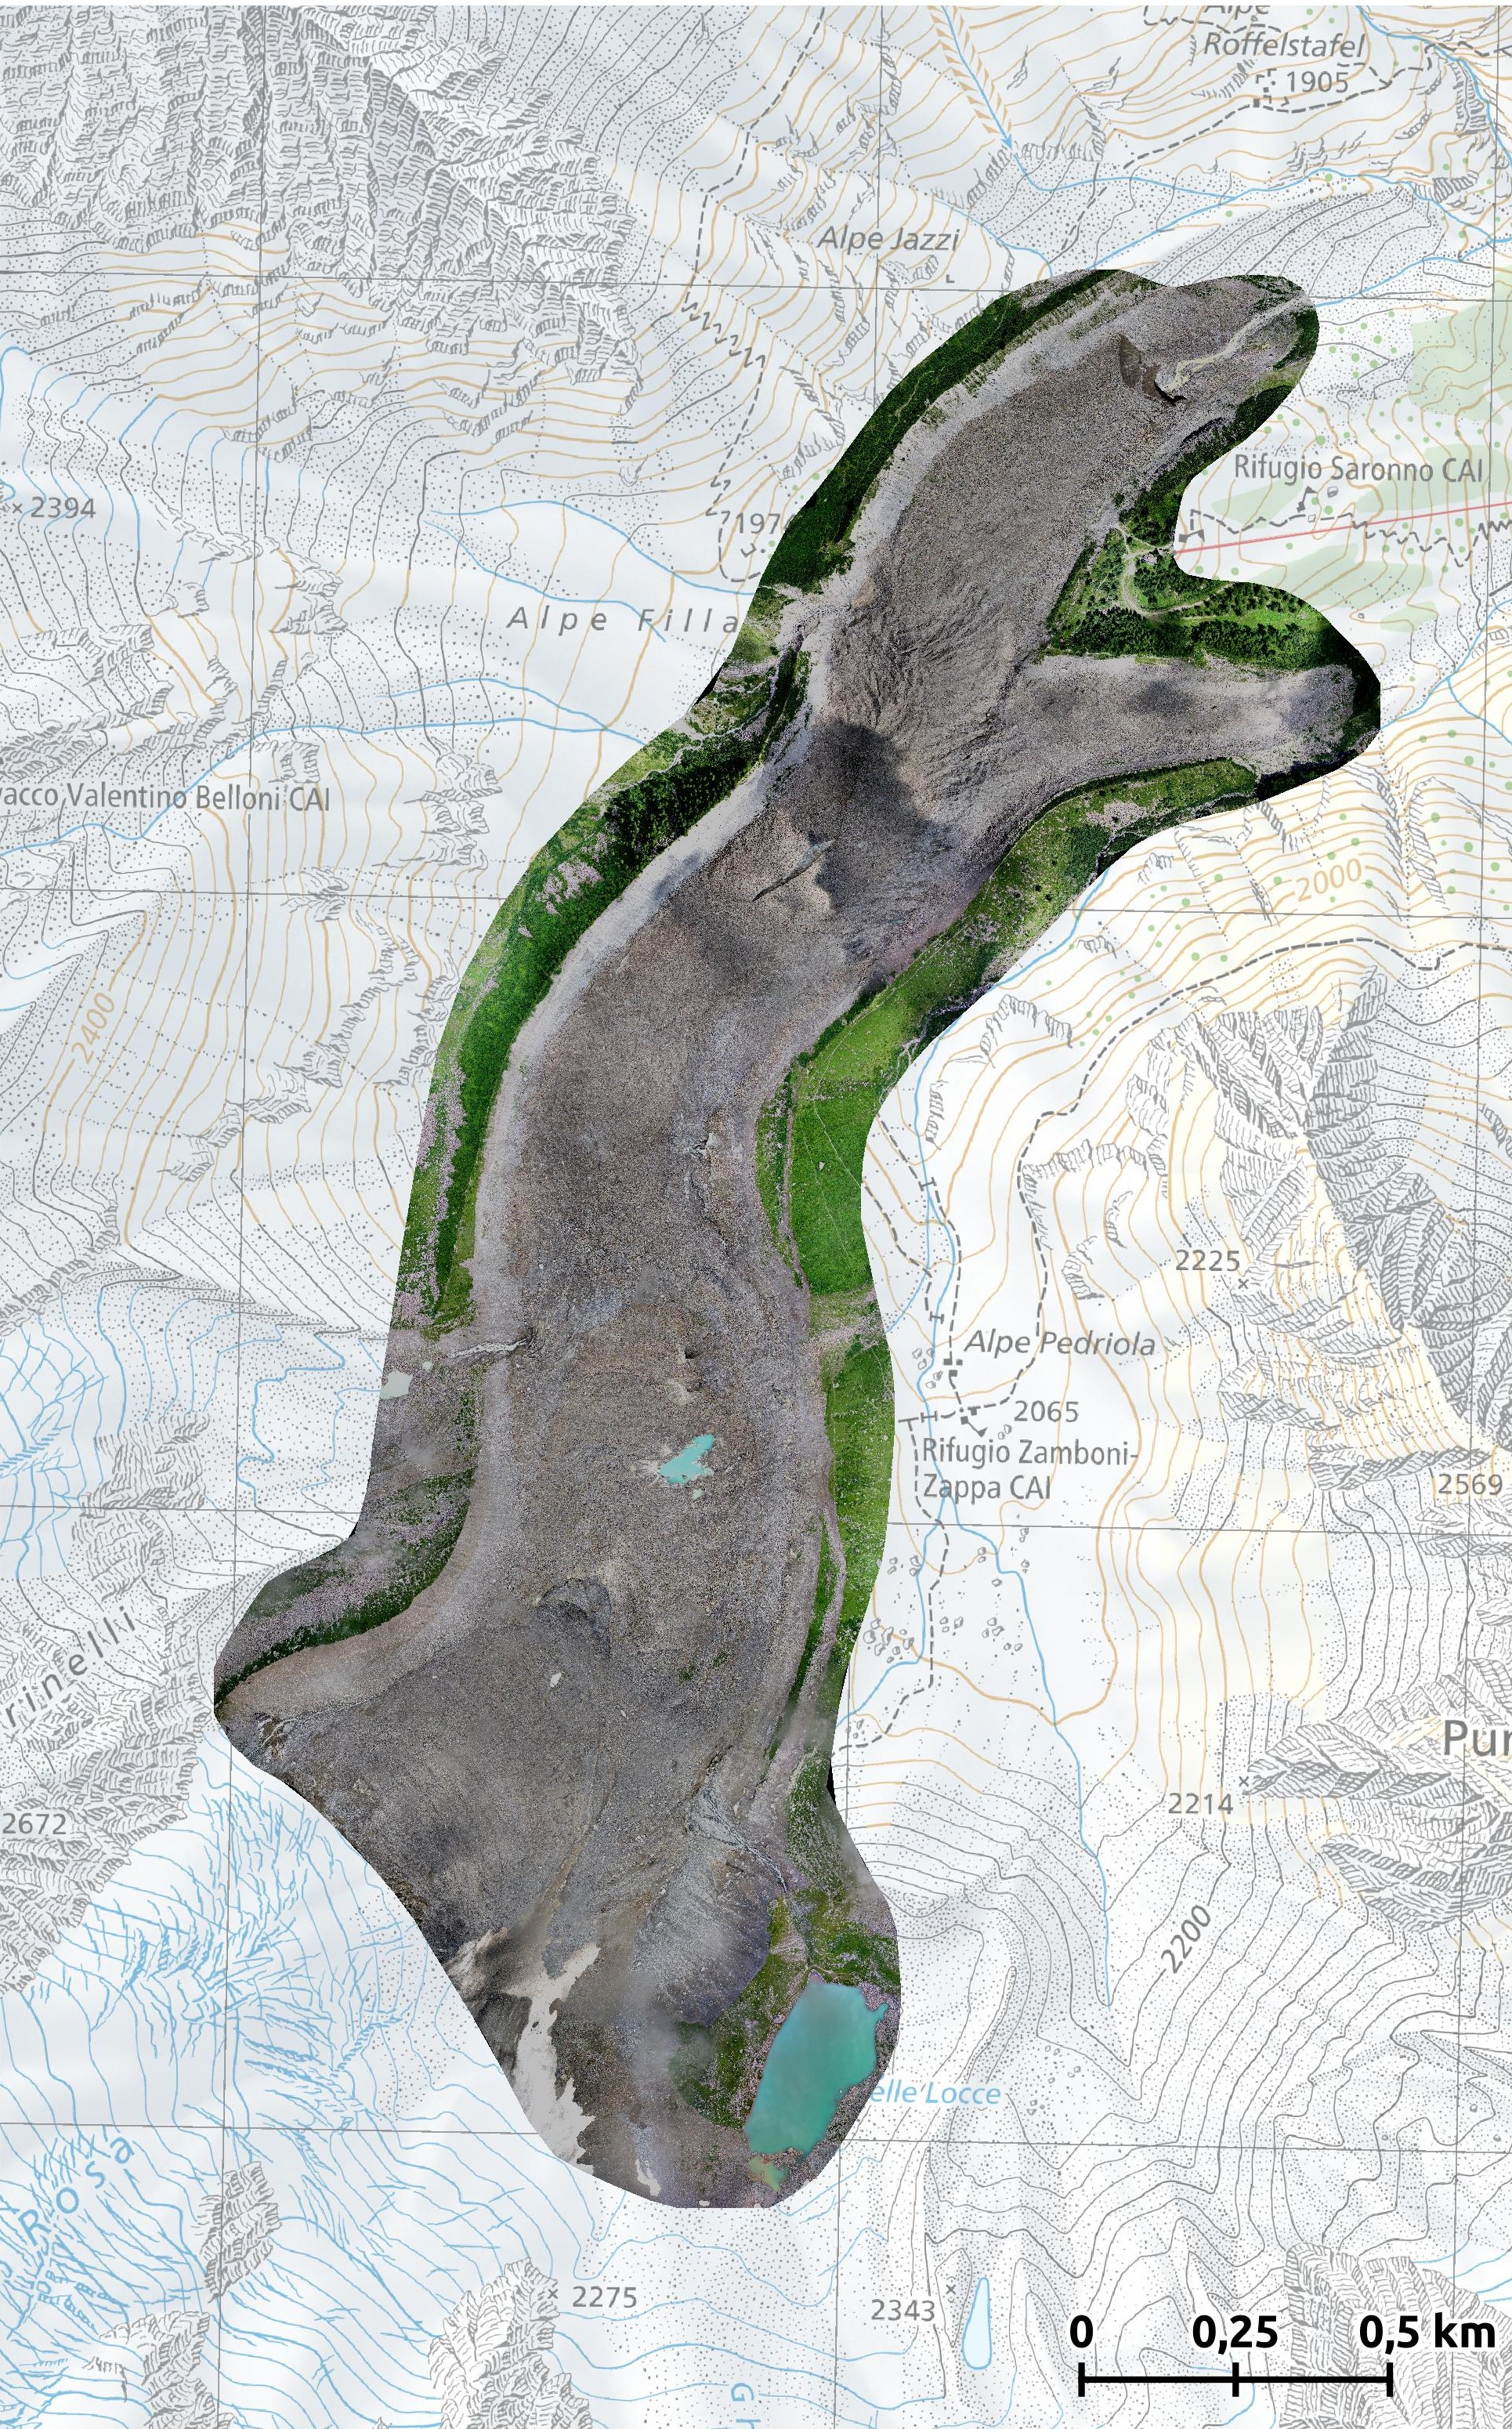
\includegraphics[width=\textwidth]{figures/appendix/orto_2021.jpg}
    \caption{UAV orthophoto from 2021. Scale 1:15000}
\end{figure}

\begin{figure}[p]
    \centering
    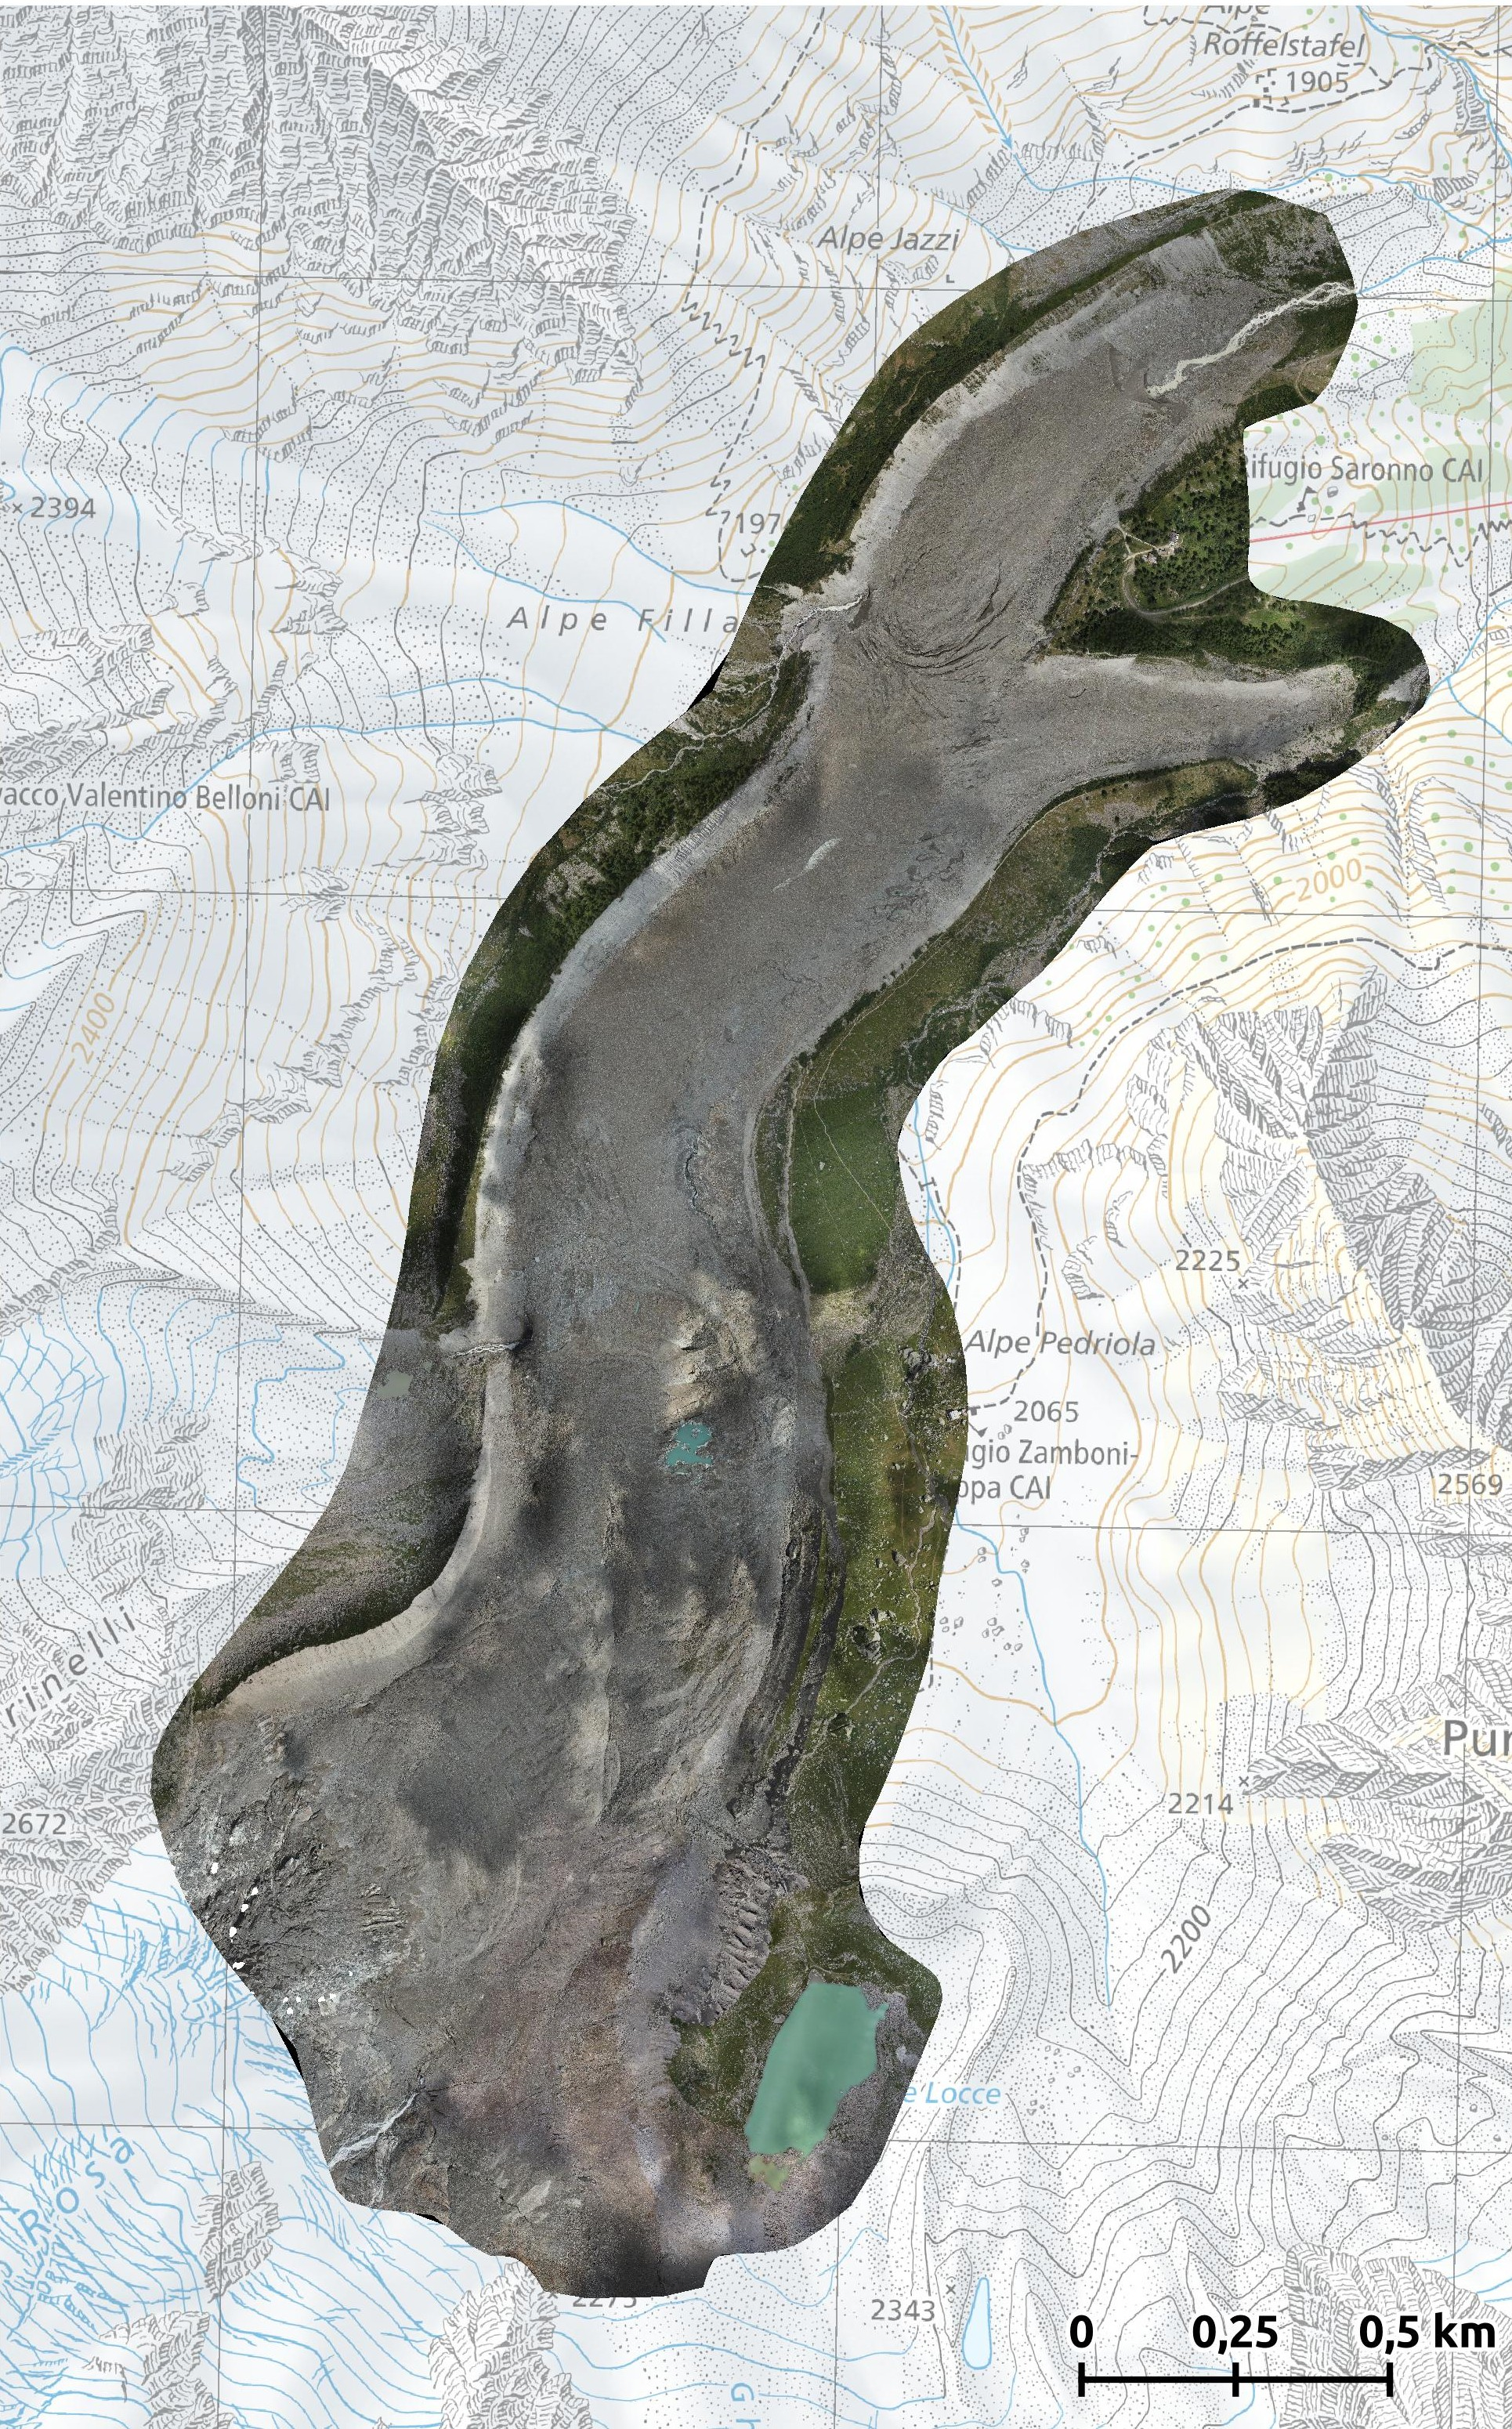
\includegraphics[width=\textwidth]{figures/appendix/orto_2022.jpg}
    \caption{UAV orthophoto from 2022. Scale 1:15000}
\end{figure}

\begin{figure}[p]
    \centering
    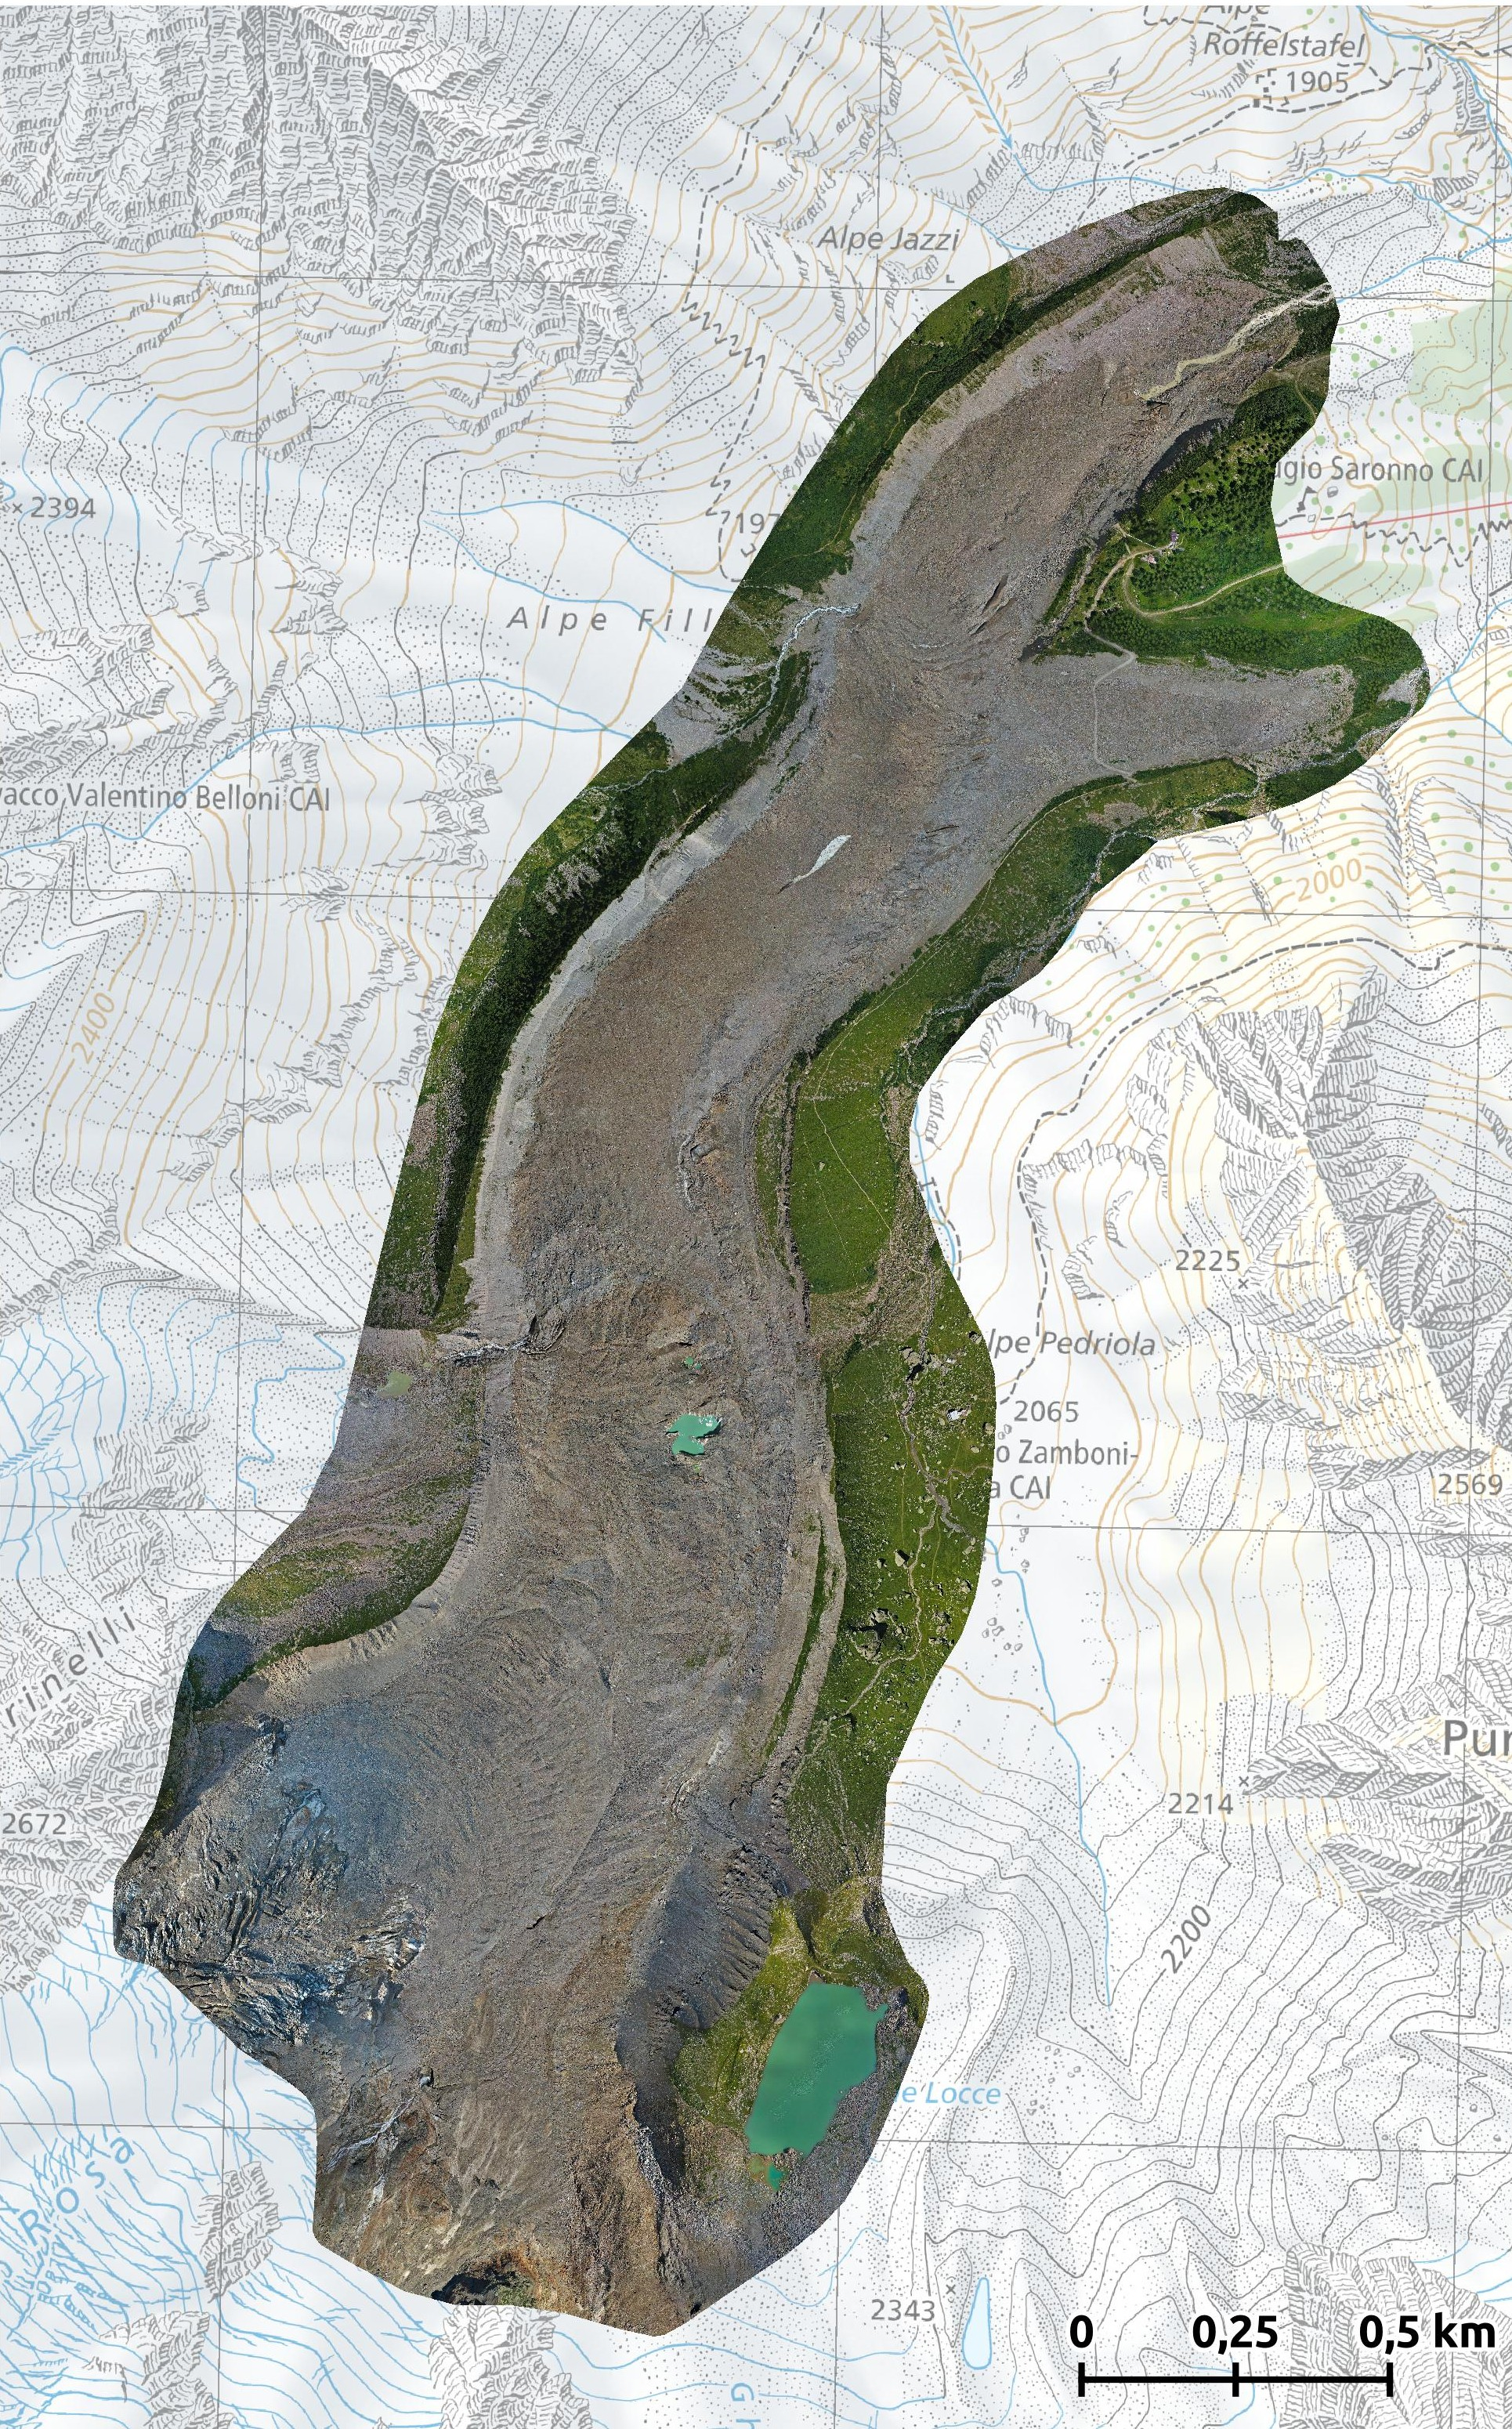
\includegraphics[width=\textwidth]{figures/appendix/orto_2023.jpg}
    \caption{UAV orthophoto from 2023. Scale 1:15000}
\end{figure}

% \chapter{DSMs}\label{app:dsm}

% \begin{figure}[p]
%     \centering
%     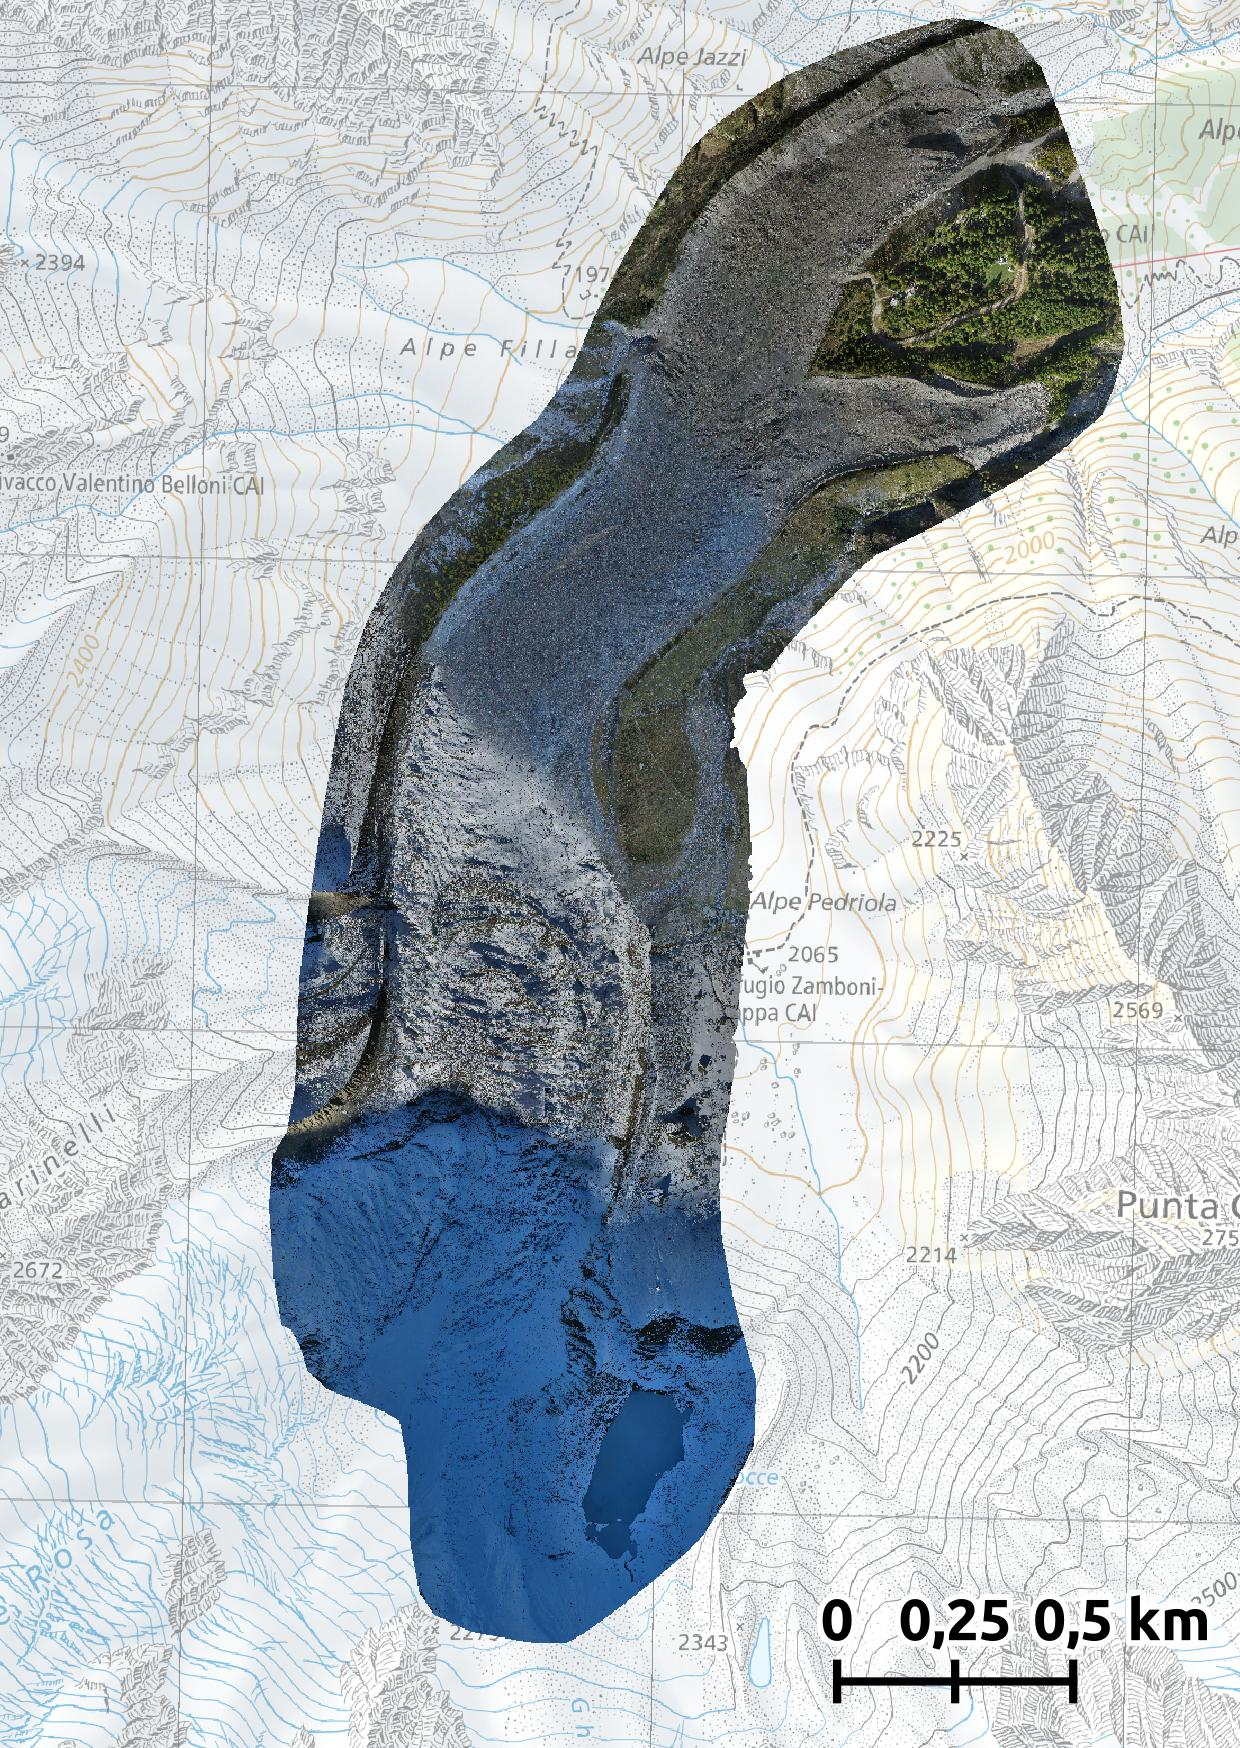
\includegraphics[width=\textwidth]{figures/chapter3/orto2015.jpg}
%     \caption{UAV-based orthophoto 2015}
% \end{figure}

% \begin{figure}
%     \centering
%     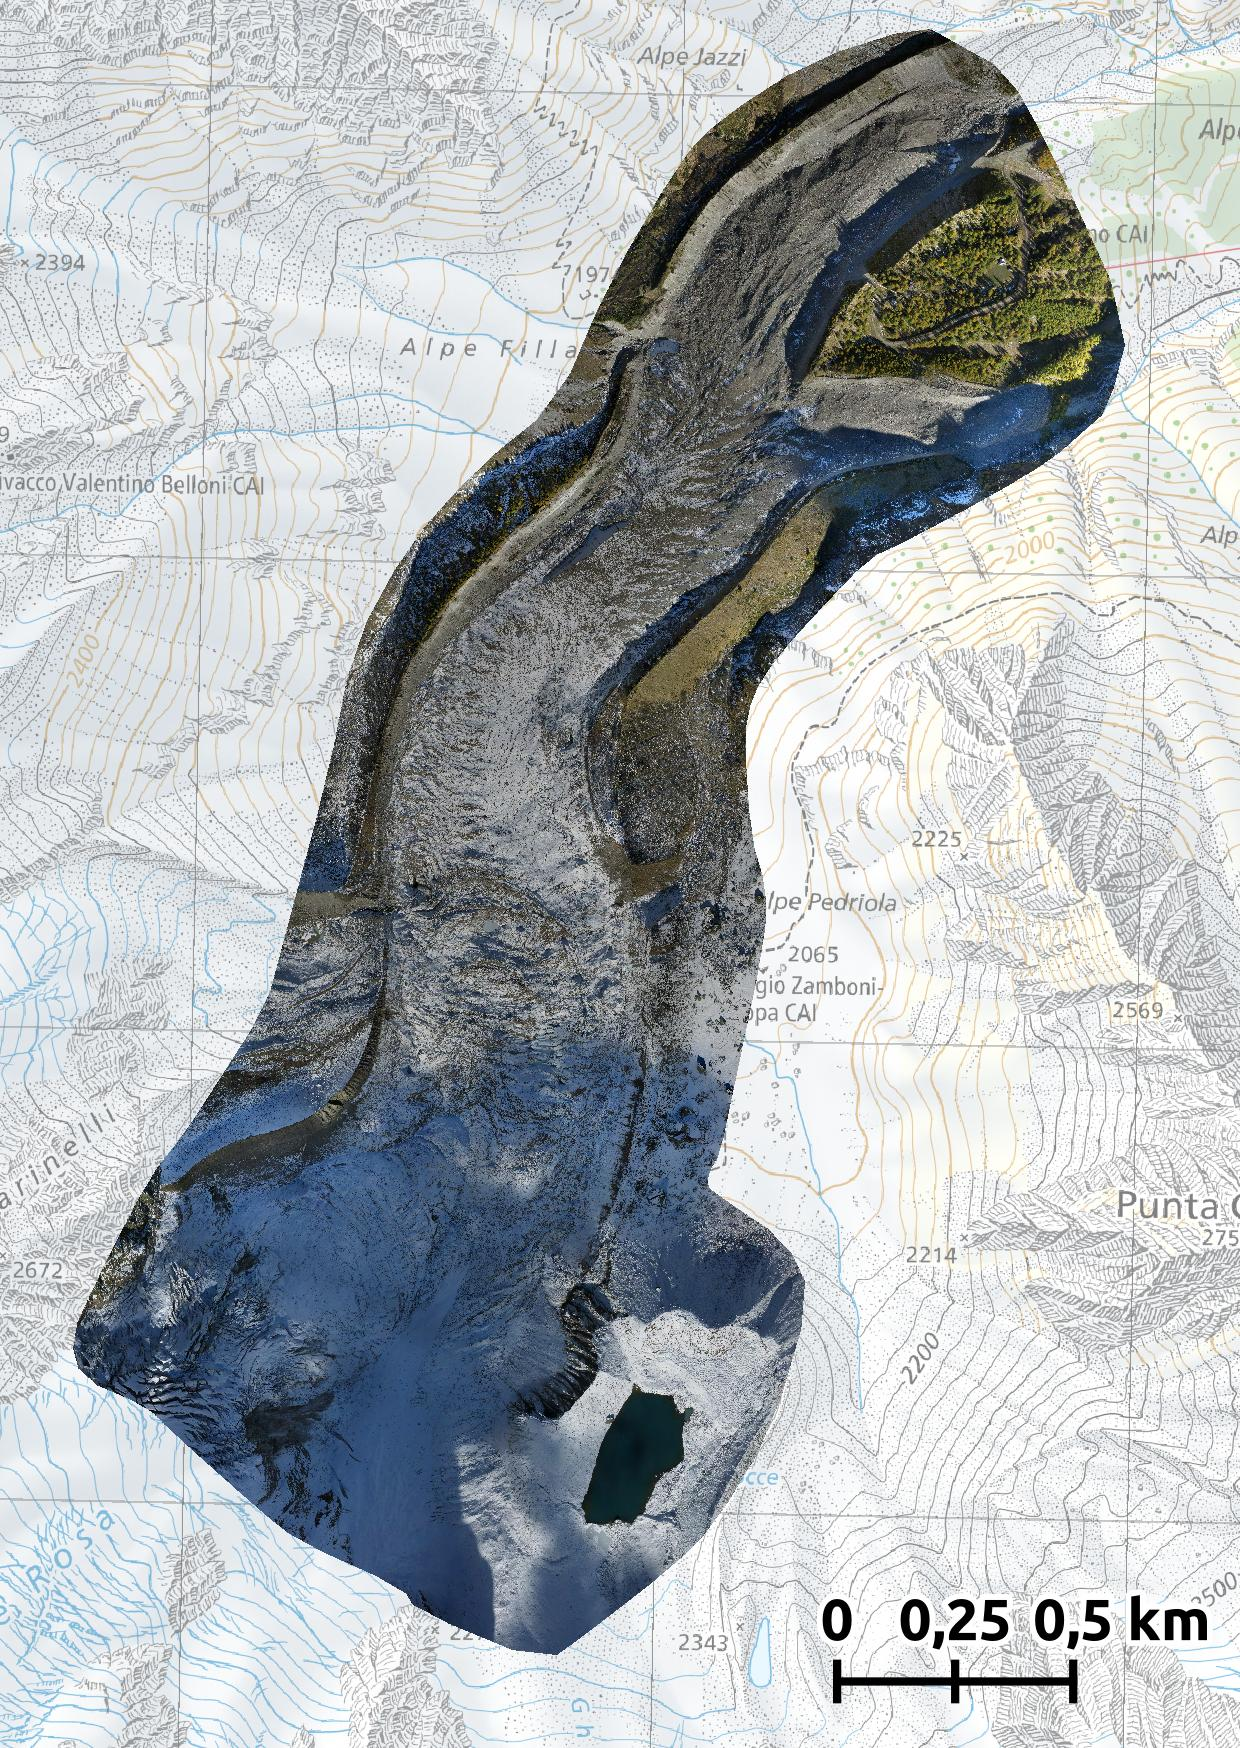
\includegraphics[width=\textwidth]{figures/chapter3/orto2016.jpg}
% \end{figure}

\chapter{Surface velocity fields 2015-2023}\label{app:sfv}

\begin{figure}[p]
    \centering
    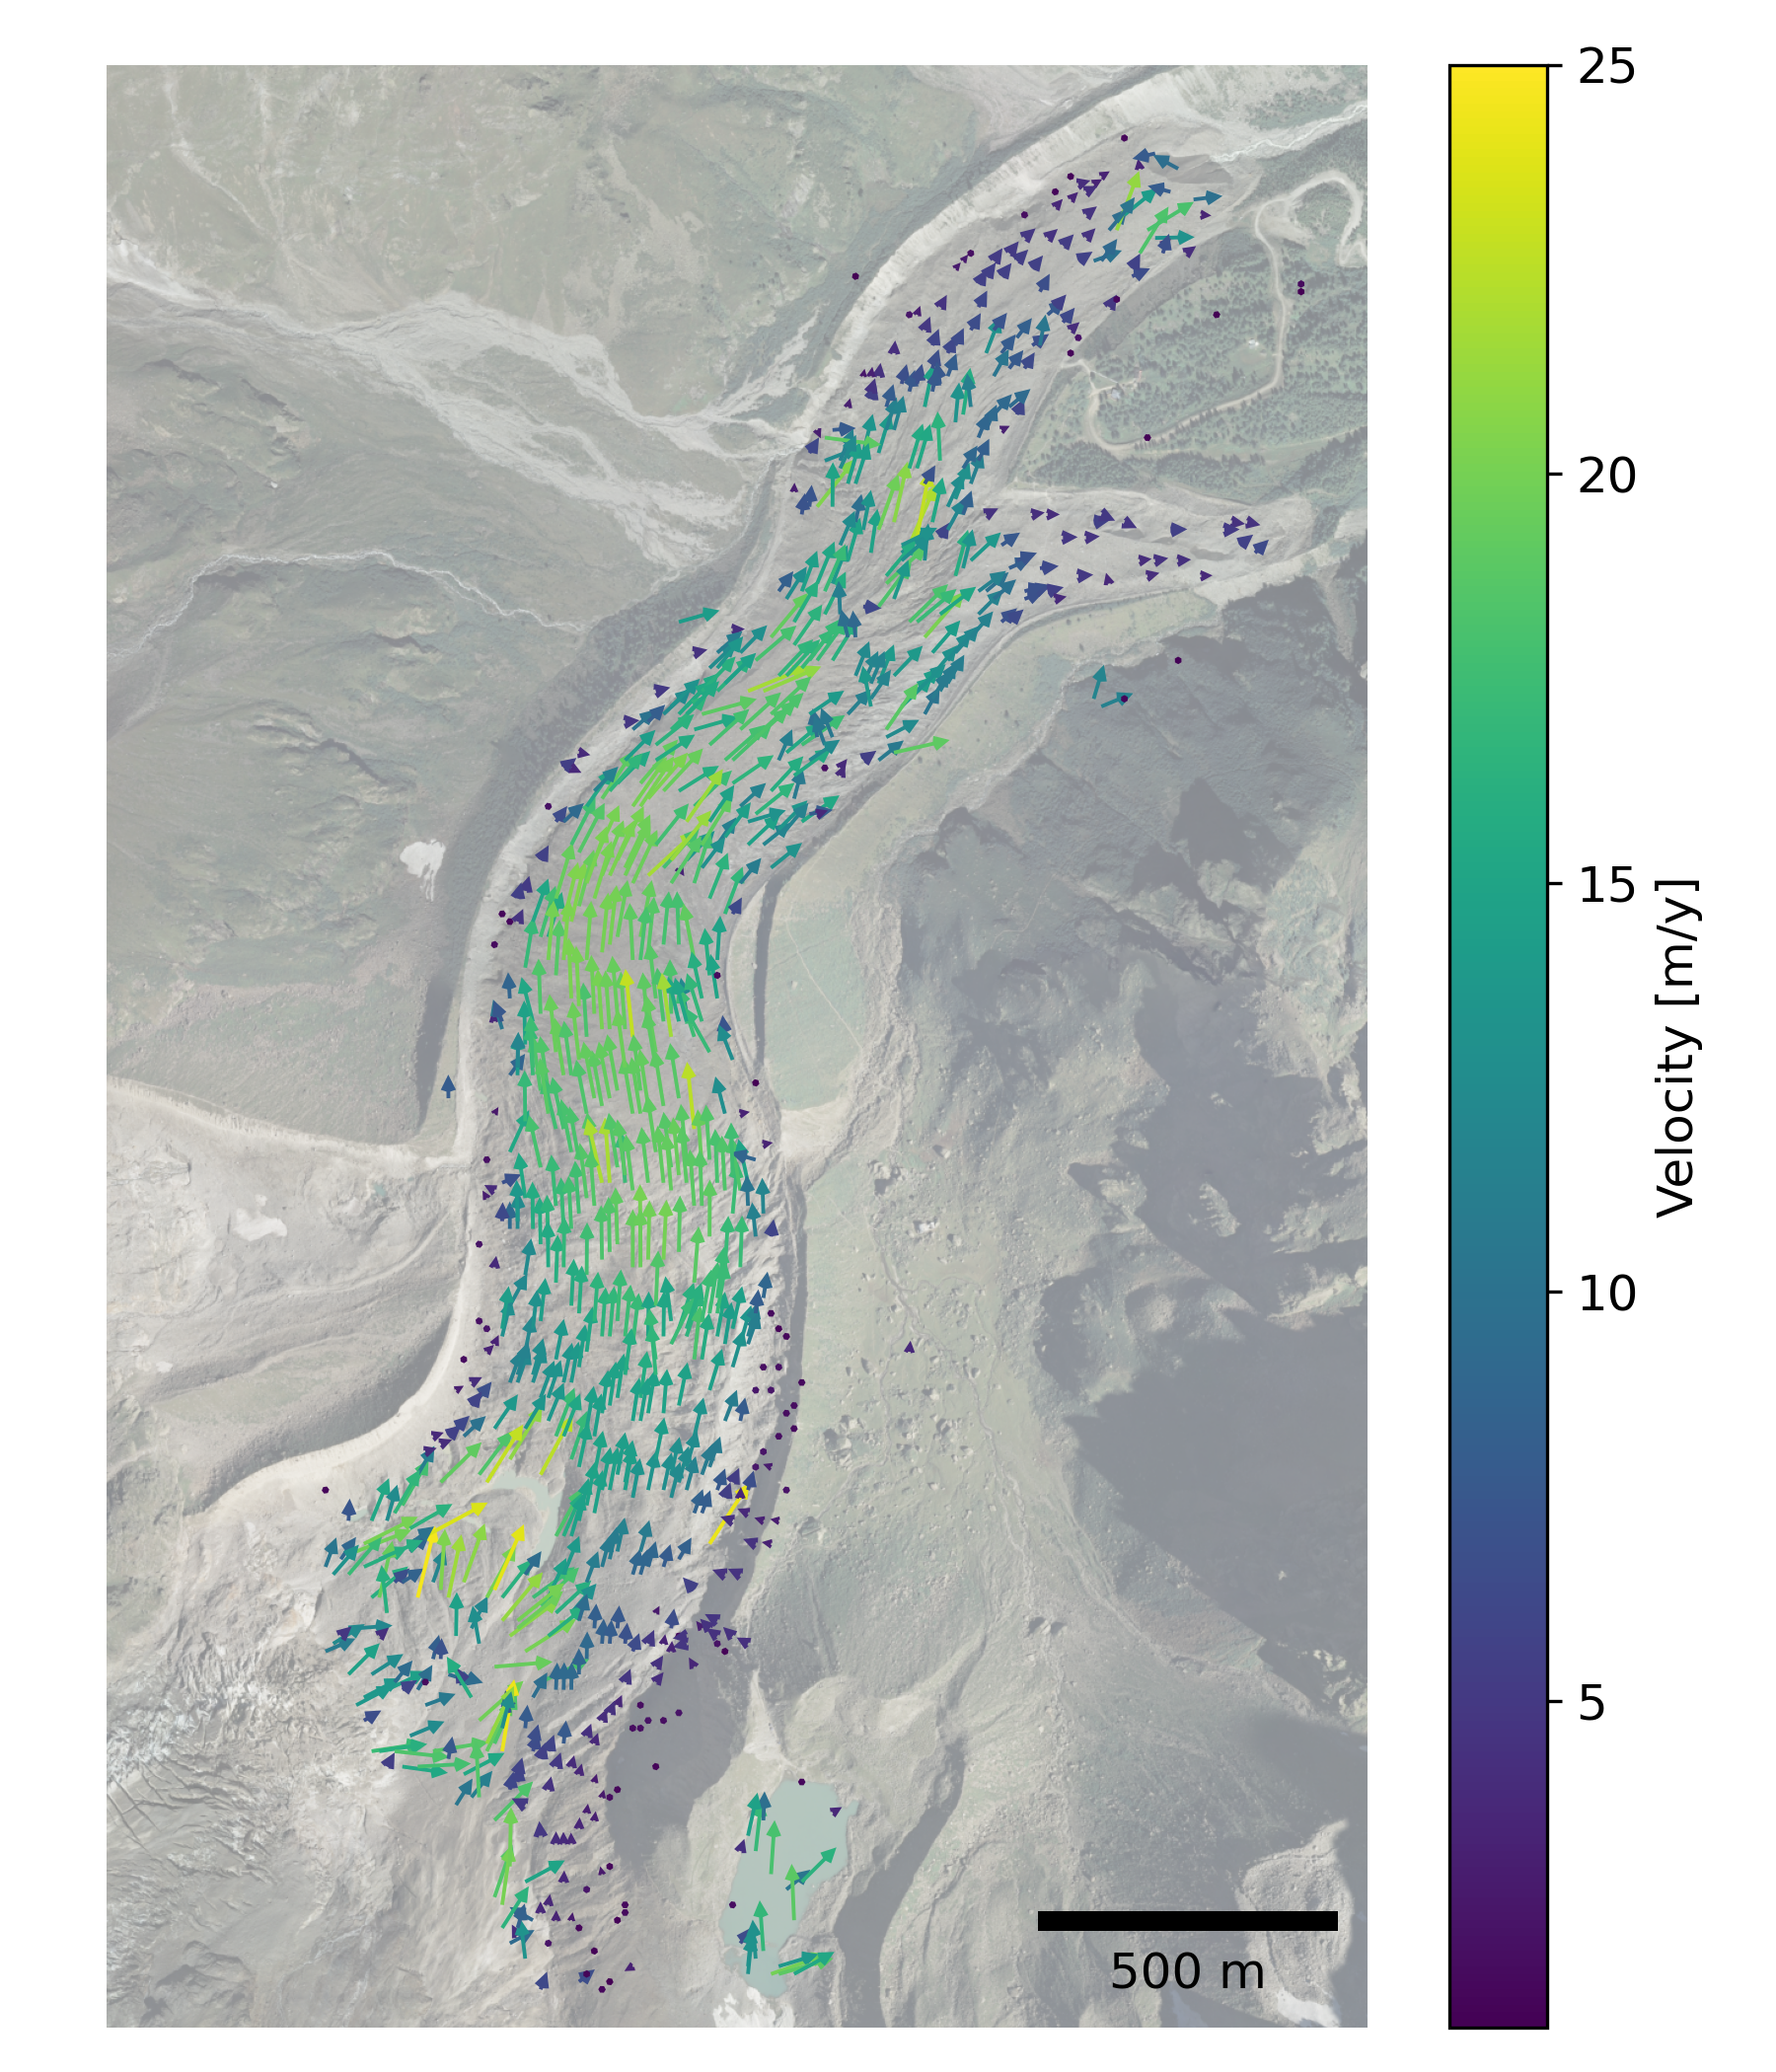
\includegraphics[width=\textwidth]{figures/chapter3/velocity_DIC_2015-2016.png}
    \caption{Glacier surface velocity field derived by DIC on DSM 2015-2016}
\end{figure}

\begin{figure}
    \centering
    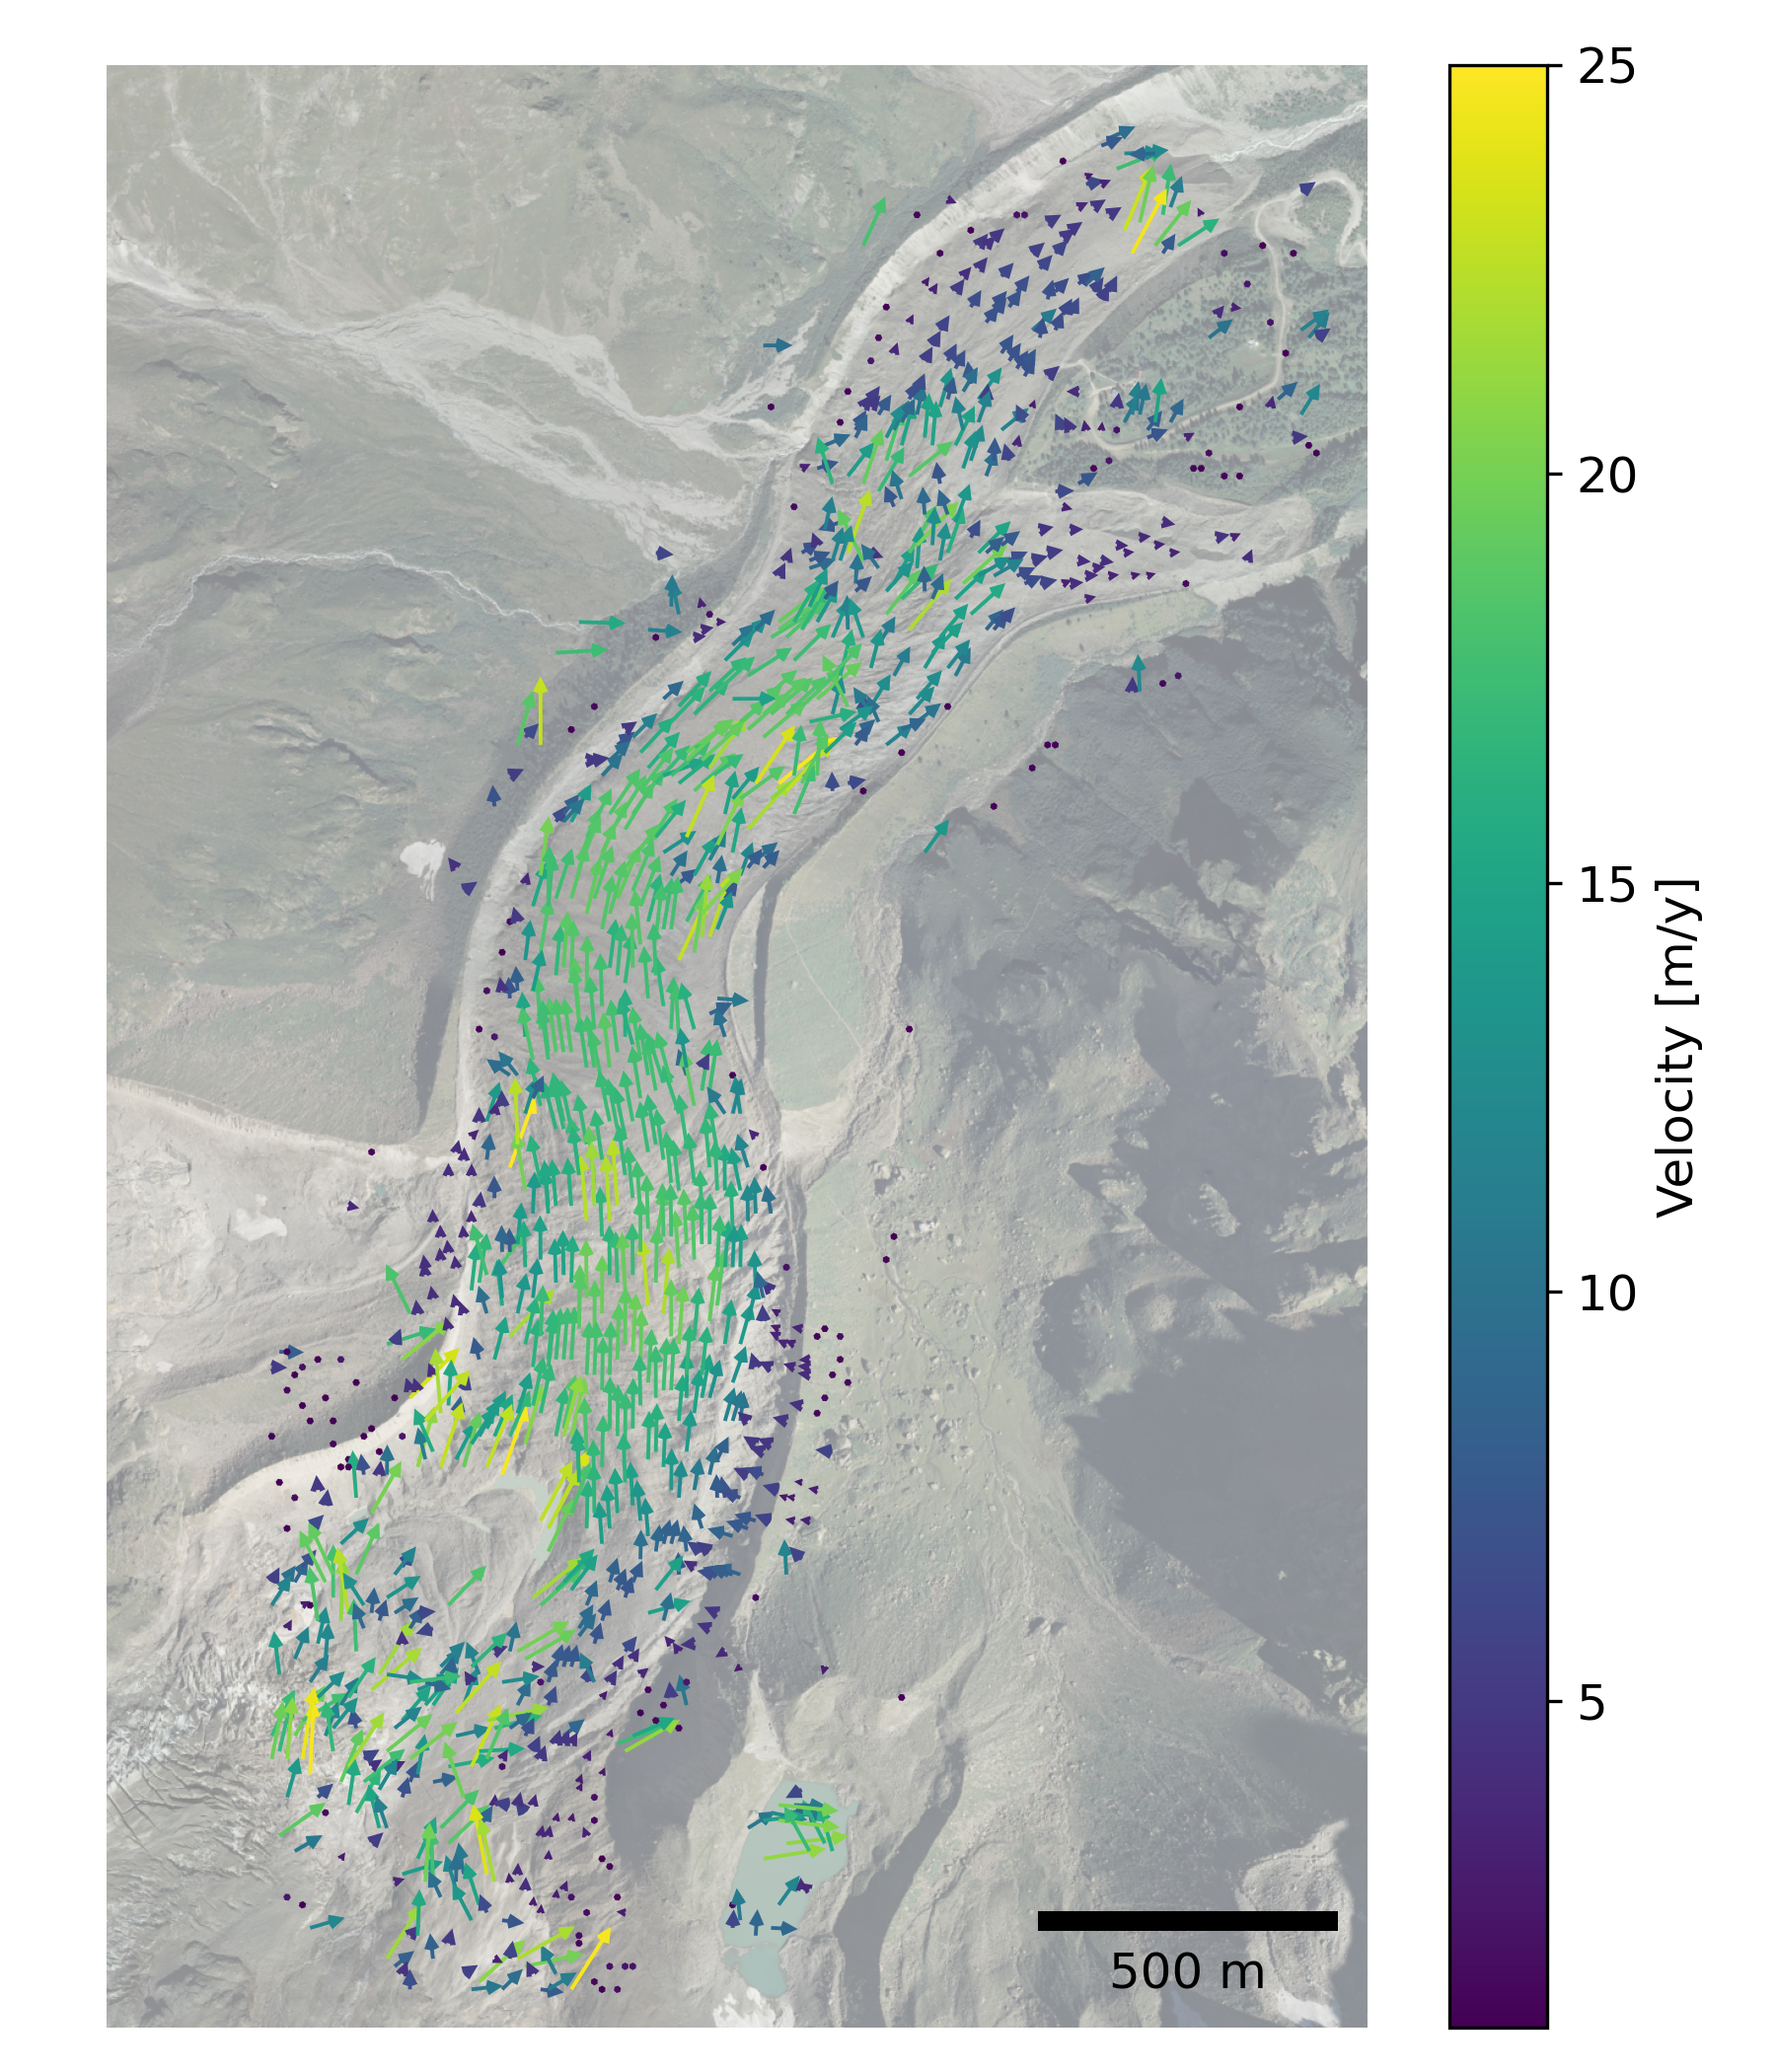
\includegraphics[width=\textwidth]{figures/chapter3/velocity_DIC_2016-2017.png}
\end{figure}


\chapter{Cross-sections}\label{app:xsec}

\begin{figure}[p]
    \centering
    \includegraphics[width=\textwidth]{figures/chapter3/profiles_map.png}\\
    \caption{Location of the cross-sections}
\end{figure}

\begin{figure}[p]
    \centering
    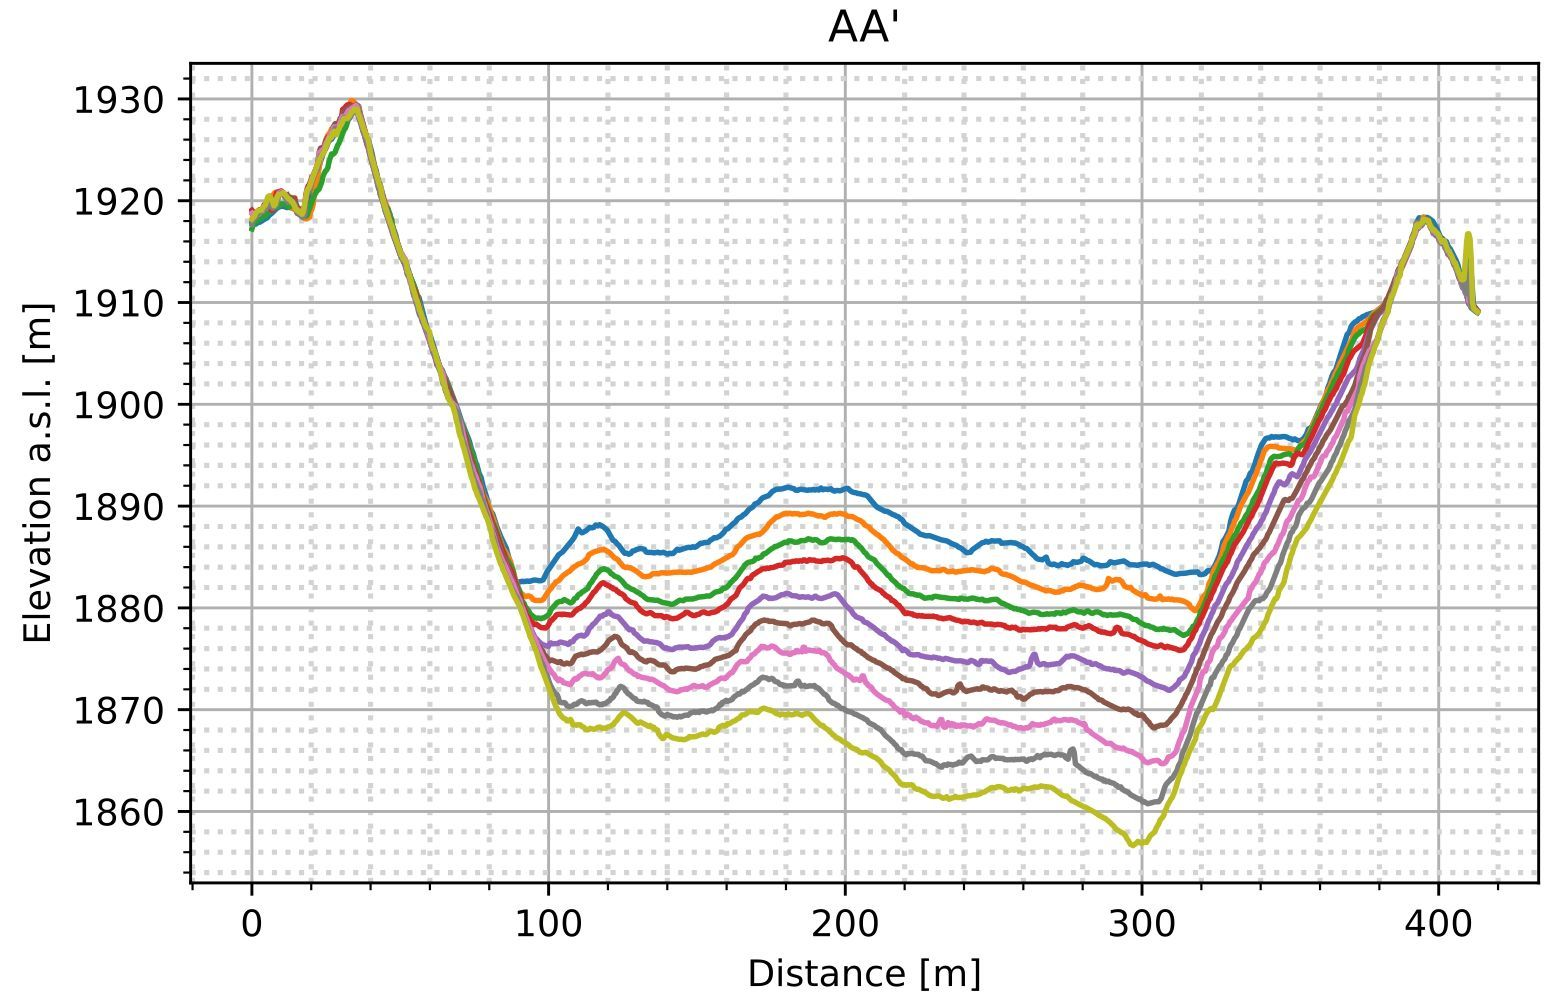
\includegraphics[width=\textwidth]{figures/appendix/profile_A.jpg}\\
    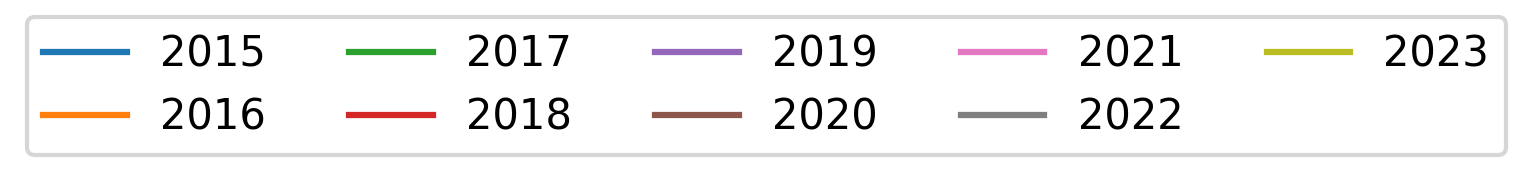
\includegraphics[width=0.7\textwidth]{figures/chapter3/profiles_legend.png}
    \caption{Cross sections along the profile AA'}
\end{figure}

\begin{figure}[p]
    \centering
    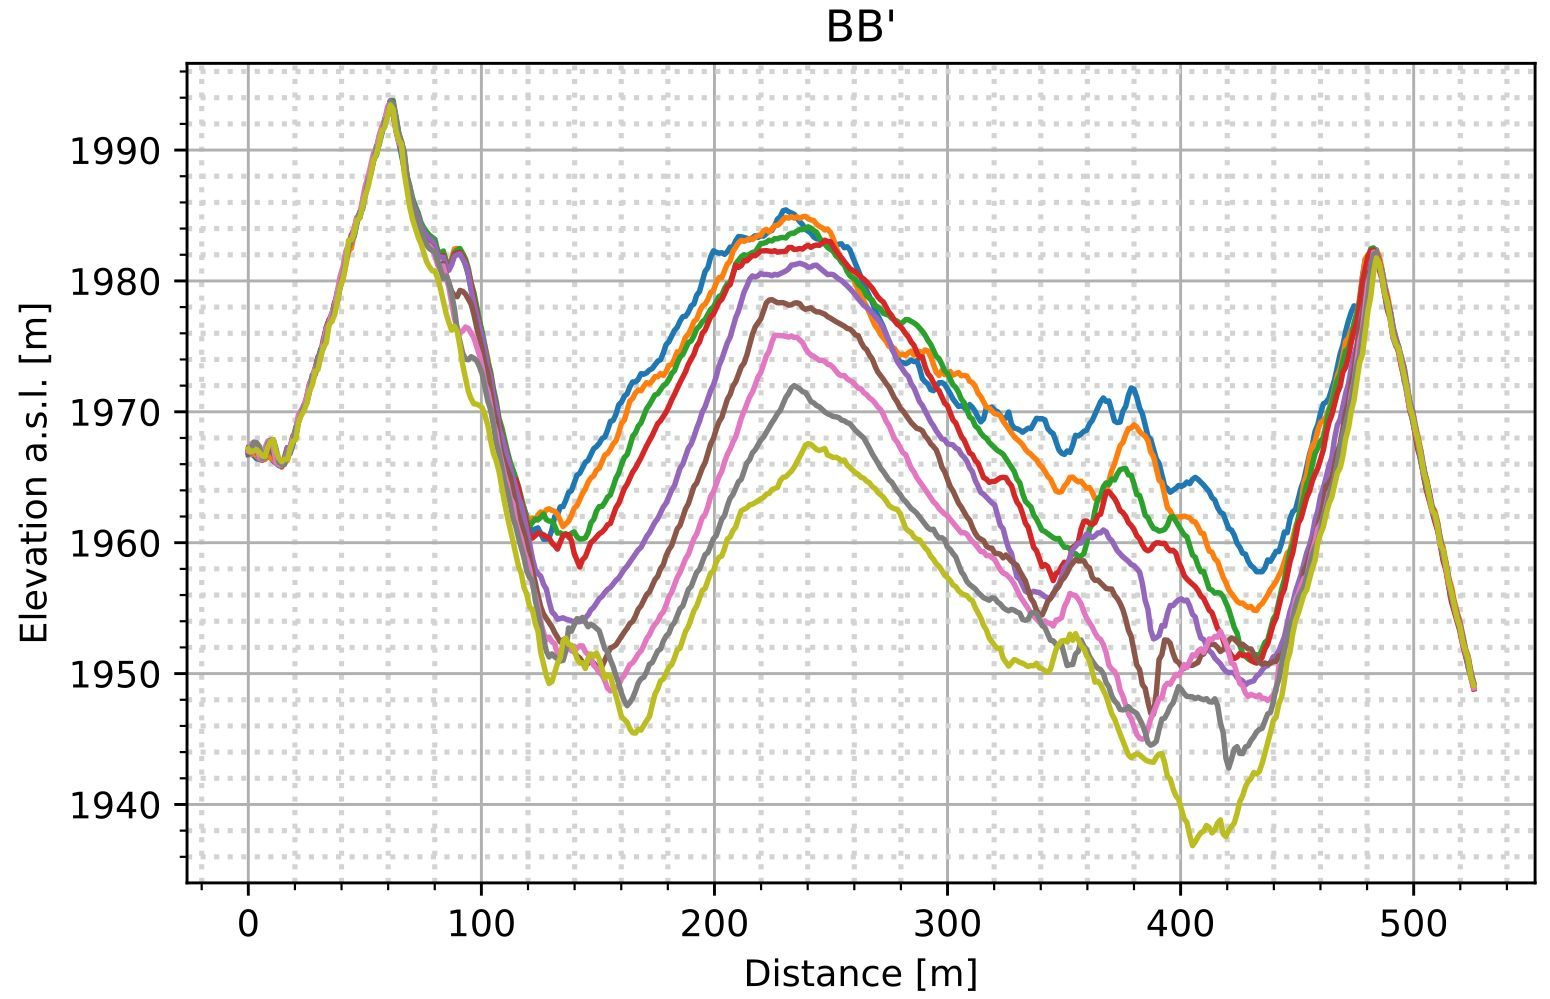
\includegraphics[width=\textwidth]{figures/appendix/profile_B.jpg}\\
    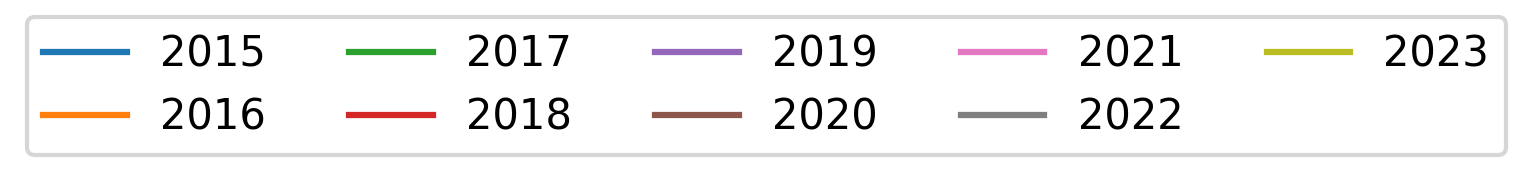
\includegraphics[width=0.7\textwidth]{figures/chapter3/profiles_legend.png}
    \caption{Cross sections along the profile BB'}
\end{figure}

\begin{figure}[p]
    \centering
    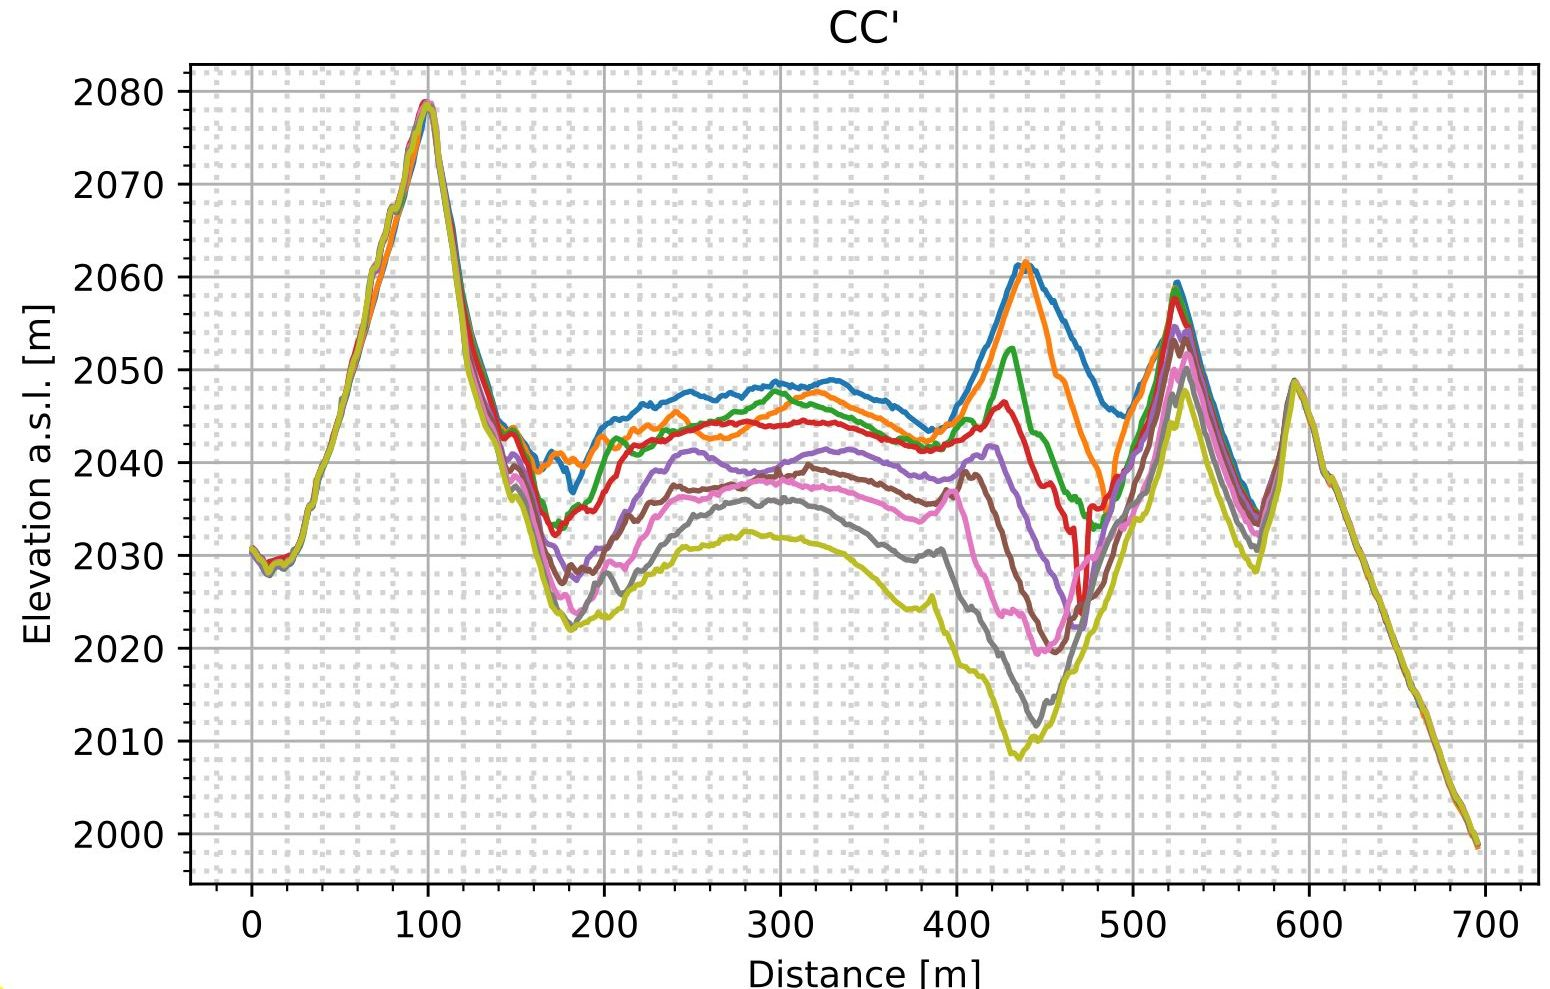
\includegraphics[width=\textwidth]{figures/appendix/profile_C.jpg}\\
    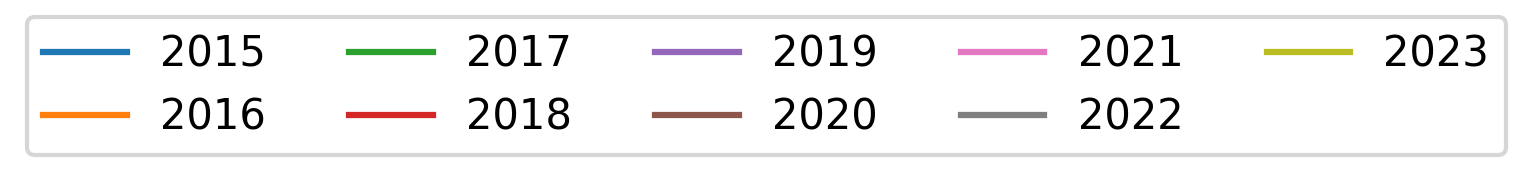
\includegraphics[width=0.7\textwidth]{figures/chapter3/profiles_legend.png}
    \caption{Cross sections along the profile CC'}
\end{figure}

\begin{figure}[p]
    \centering
    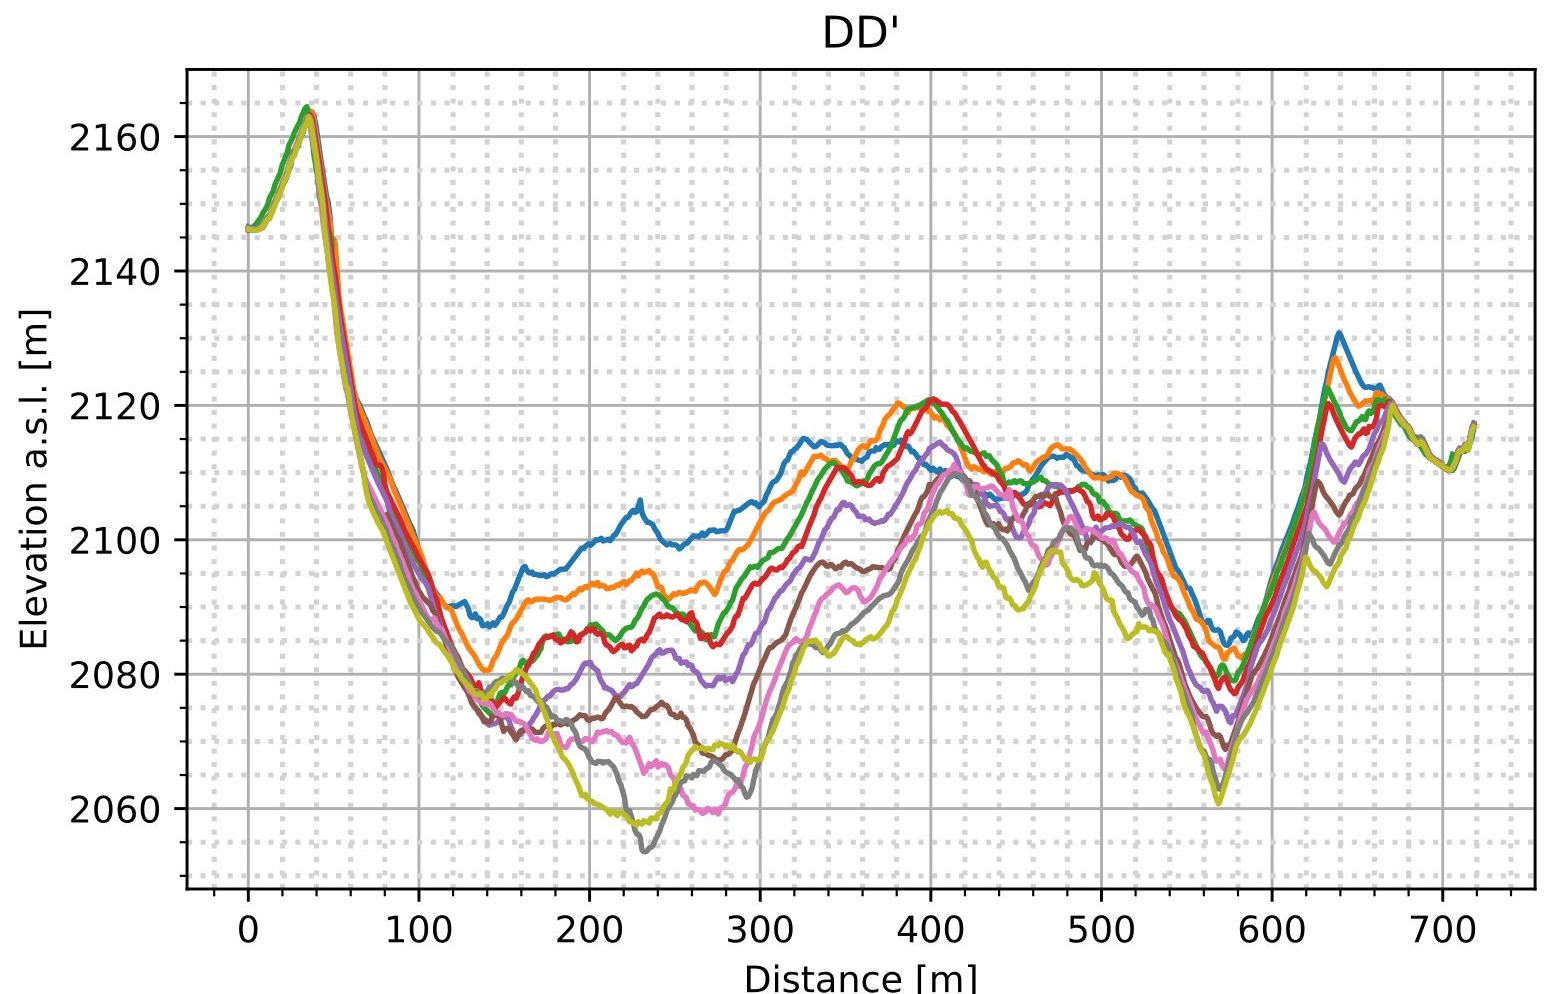
\includegraphics[width=\textwidth]{figures/appendix/profile_D.jpg}\\
    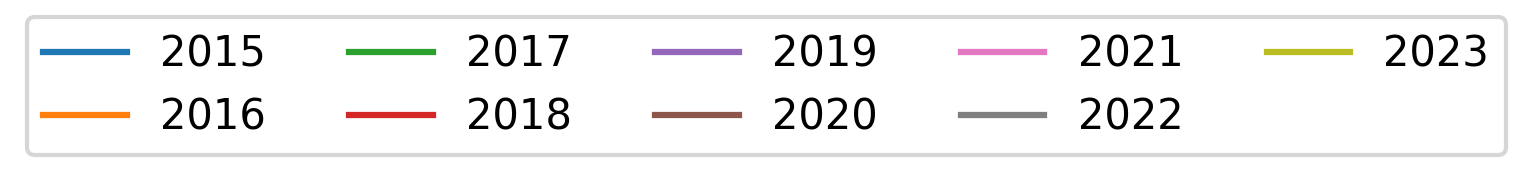
\includegraphics[width=0.7\textwidth]{figures/chapter3/profiles_legend.png}
    \caption{Cross sections along the profile DD'}
\end{figure}

\begin{figure}[p]
    \centering
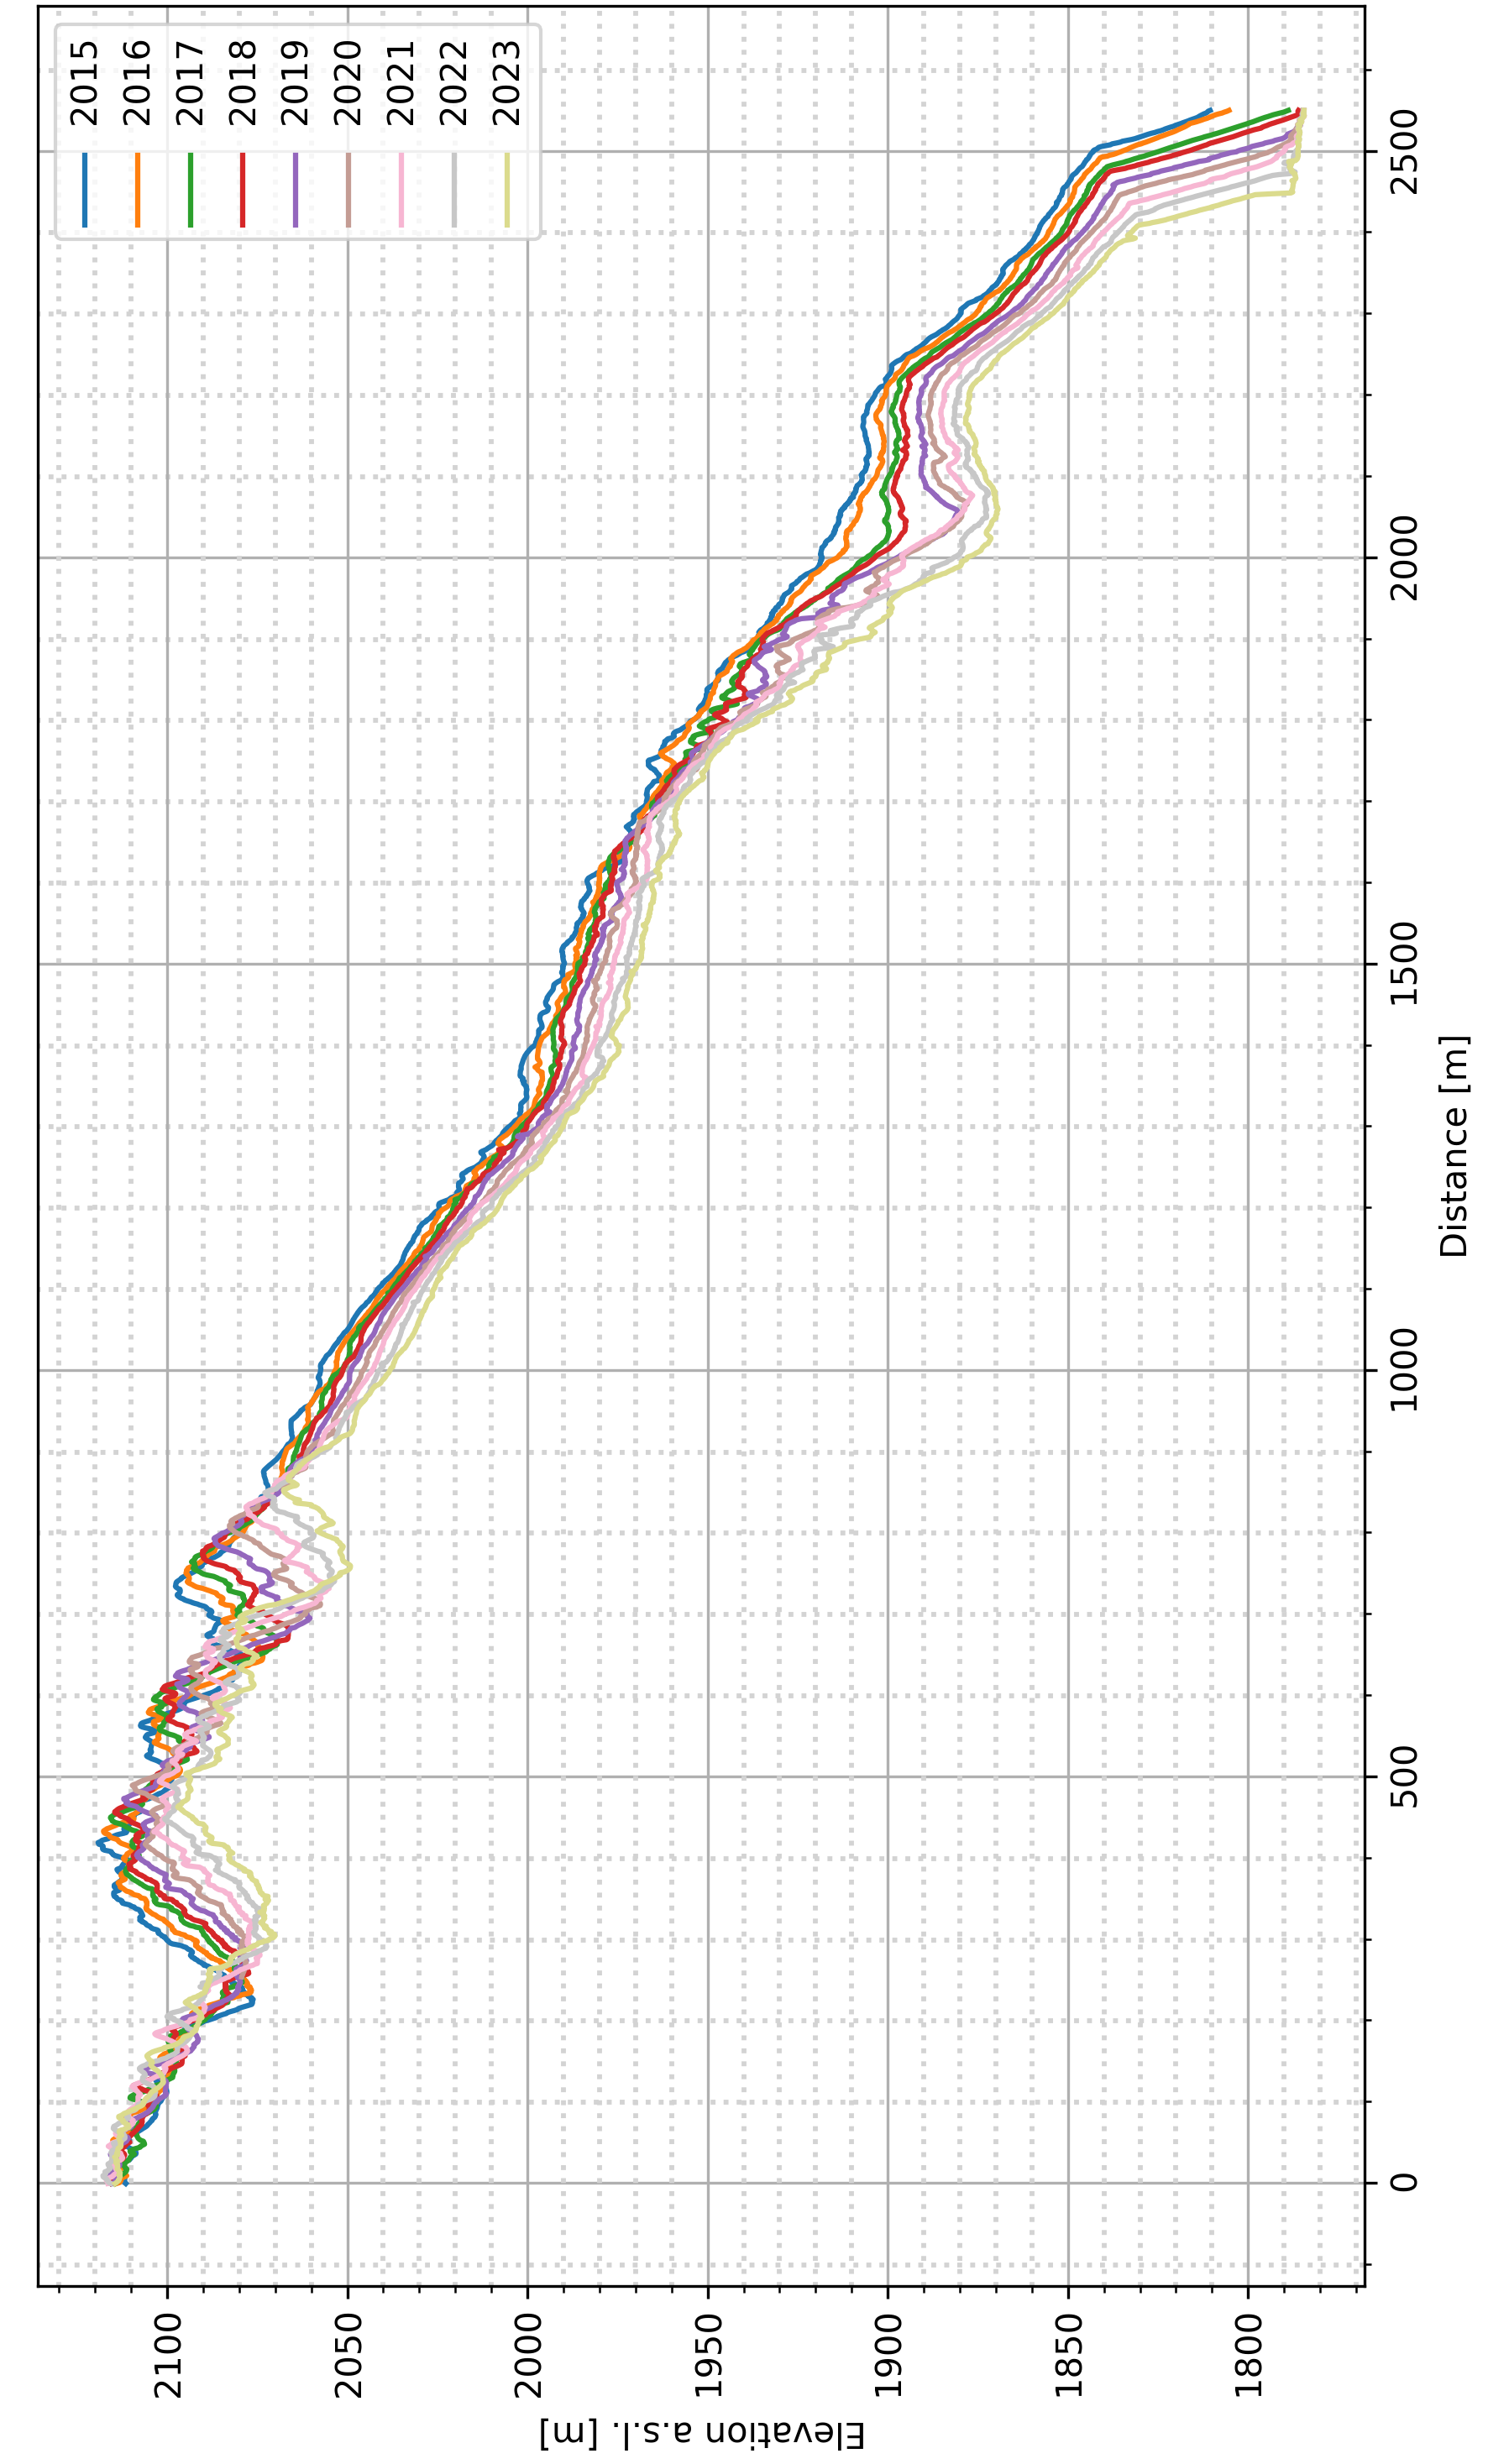
\includegraphics[width=0.9\textwidth]{figures/appendix/profile_flow_rot.png}
    \caption{Cross sections along the profile EE', extracted along the glacier flow direction.}
\end{figure}

